\documentclass[utf8, seminar]{fer}
%\documentclass[utf8, zavrsni, upload]{fer}
\usepackage{booktabs}
\usepackage{indentfirst}
\usepackage{subcaption}
\usepackage{placeins}
\usepackage{float}
\usepackage{cite} % Za bibliografiju
\usepackage{url} % Za web adrese
\usepackage{listings}
\usepackage{caption}
\usepackage{tabularx}
\usepackage{amsmath}
\usepackage{amsfonts}
\usepackage{amssymb}
\usepackage{amsthm}
\usepackage{mathtools}
\usepackage{graphicx}
\usepackage{booktabs}
\usepackage{array}
\usepackage{longtable}
\usepackage{hyperref}
\usepackage{url}
\usepackage{fancyhdr}
\usepackage{setspace}
\usepackage{titlesec}
\usepackage{enumitem}
\usepackage{xcolor}
\setlocalecaption{croatian}{abstract}{Sažetak}

\usepackage{mathptmx} % Use Times New Roman font
\usepackage{setspace} % For setting line spacing
\singlespacing% Set line spacing to 1

% Smanjeni razmak između bullet-a
\setlist[itemize]{itemsep=0pt, parsep=0pt, topsep=0pt, partopsep=0pt}
\setlist[enumerate]{itemsep=0pt, parsep=0pt, topsep=0pt, partopsep=0pt}

\usepackage{titlesec} % To control the title spacing
\titlespacing*{\chapter}{0pt}{-30pt}{10pt}

\renewcommand{\figurename}{Slika}
\renewcommand{\bibname}{Literatura}
\renewcommand{\tablename}{Tablica}
\renewcommand{\contentsname}{Sadržaj}
\renewcommand\thepage{}

\title{Comparison of EDR tools}
\naslov{Usporedba alata za nadzor i intervenciju na krajnjim točkama (Endpoint Detection and Response)}
\brojrada{N/a}
\author{Ante Čavar}
\datum{lipanj, 2025.}
\mentor{prof.dr.sc. Stjepan Groš}

\begin{document}
\maketitle
% \zadatak{hr_0036540817_73.pdf}
\begin{zahvale}
Zahvaljujem se prijateljima i obitelji koji su mi bili podrška prilikom pisanja ovog rada.
\end{zahvale}
\newpage
\tableofcontents
\newpage
\mainmatter%
\setcounter{page}{1}
\renewcommand\thepage{\arabic{page}}
% \chapter{Uvod}
\par Sigurnost web aplikacija je bitan dio razvoja moderne programske potpore. 
Kako se napadi na web aplikacije povećavaju iz dana u dan, potrebno je osim razumijevanja 
prijetnji i ranjivosti, imati i alate kojima ranjivosti a s njima i prijetnje možemo svesti na prihvatljivi minimum.

% \par Dva najraširenija takva alata trenutno dostupna javnosti su OWASP ZAP i Burp 
% Suite. OWASP ZAP (još znan i kao Zed Attack Proxy) je program otvorenog koda namijenjen
% za skeniranje web aplikacija tj.\ stranica. Produkt je organizacije \textit{Open Web Application 
% Security Project} (OWASP) te održavan kako od njih tako i od nemale skupine programera 
% i sigurnosnih stručnjaka iz cijelog svijeta. Alat pruža široki skup mogućnosti 
% za detekciju i testiranje ranjivosti u web aplikacijama. 

% \par Uz ZAP postoji Burp Suite, stariji i komercijalni alat namijenjen za sigurnosno testiranje 
% web aplikacija. Burp suite je razvila kompanija PortSwigger koja se također brine za njegovo 
% održavanje. Burp suite omogućuje pristup velikom rasponu alata, od skenera za traženje ranjivosti 
% pa sve do naprednih alata za \textit{fuzzing} i analizu web aplikacija. Najpoznatiji 
% alat među njima je \textit{proxy} koji omogućava korisnicima da presretnu HTTP/S zahtjeve 
% te izmijene HTTP/S zahtjeve i odgovore.

% \par OWASP ZAP i Burp Suite igraju važnu ulogu u području sigurnosti web aplikacija. 
% Prethodno navedeni i slični alati pomažu razvojnim inženjerima i sigurnosnim specijalistima u identifikaciji ranjivosti,
% razumijevanju površine napada (engl. \textit{attack surface}), vektora napada (engl. \textit{attack vector}) te u
% implementaciji efektivnih sigurnosnih rješenja.

% \par Cilj ovog rada je istražiti alat OWASP ZAP kao potencijalnu zamjenu za Burp Suite Professional testirajući
% mogućnosti oba alata u podjednakim uvjetima.
U ovom radu će se usporediti dva najraširenija alata za skeniranje i testiranje sigurnosti web aplikacija: OWASP ZAP i Burp Suite. 
Cilj je identificirati razlike u funkcionalnostima između ova dva alata, istražiti kako se mogu nadomjestiti funkcionalnosti koje ZAP 
nema, te opisati kako se pišu dodaci i proširuju mogućnosti ZAP-a. Na kraju, testirat će se nekoliko laboratorijskih vježbi koje se 
inače rješavaju pomoću alata Burp suite, koristeći ZAP.

Burp Suite je moćan, ali komercijalan alat koji zahtijeva skupu licencu za pristup svim funkcionalnostima. 
Za potrebe istraživanja i učenja, ovaj trošak može biti značajan. S druge strane, OWASP ZAP je alat otvorenog koda koji je besplatan 
za korištenje, ali potencijalno slabijih mogućnosti. Usporedbom ova dva alata, može se procijeniti koliko ZAP može biti održiva 
zamjena za Burp Suite u raznim scenarijima.

Najprije će se opisati osnovne funkcionalnosti oba alata. Zatim će se provesti nekoliko testova na različitim sigurnosnim scenarijima 
koristeći oba alata. Nakon toga, analizirat će se rezultati testova i usporediti performanse i mogućnosti ZAP-a i Burp Suite-a. 
Konačno, istražit će se mogućnosti proširenja funkcionalnosti ZAP-a kroz dodatke i skripte te predložiti rješenja za funkcionalnosti 
koje Burp Suite ima, a ZAP nema i pritom objasniti koji alat odabrati i zašto.
% \chapter{Funkcionalnosti}
Kako oba alata imaju pregršt funkcionalnosti navesti ću njihove najzanimljivije i najbolje implementirane funkcionalnosti 
koje će kasnije biti uspoređene.
\section{OWASP ZAP}
OWASP ZAP (još znan i kao Zed Attack Proxy) je program otvorenog koda namijenjen
za skeniranje web aplikacija tj.\ stranica. Produkt je organizacije \textit{Open Web Application 
Security Project} (OWASP) te održavan kako od njih tako i od nemale skupine programera 
i sigurnosnih stručnjaka iz cijelog svijeta. Alat pruža široki skup mogućnosti 
za detekciju i testiranje ranjivosti u web aplikacijama. Izgled ZAPa pri njegovom pokretanju vidljiv je na slici \ref{slk:owasp_start}.
\begin{figure}[H]
    \centering
    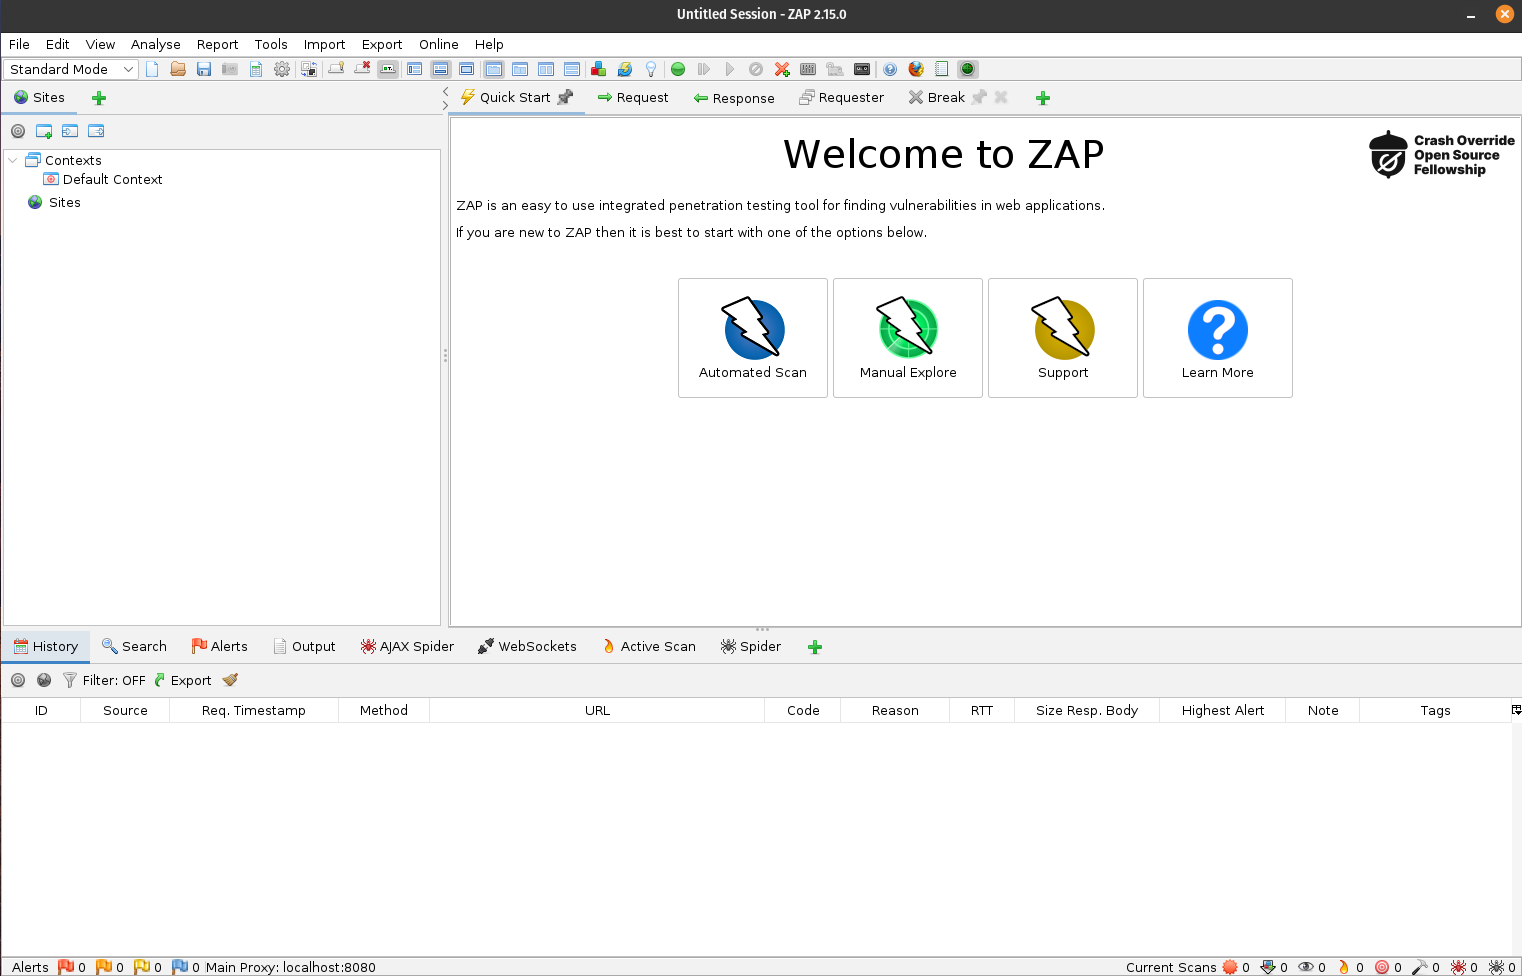
\includegraphics[width=0.8\textwidth]{slike/zap_start.png}
    \caption{Izgled OWASP ZAP-a pri pokretanju}
    \label{slk:owasp_start}
  \end{figure}

\subsection{Presretački \textit{proxy}}
\textit{Intercepting Proxy}, poznat i kao \textit{"Break"} u \textit{OWASP ZAP}-u, ključna je funkcionalnost koja omogućava 
korisnicima da presreću i pregledavaju \textit{HTTP/HTTPS} zahtjeve i odgovore između preglednika i web aplikacije. Ovo omogućuje 
korisnicima da detaljno pregledaju i modificiraju podatke prije nego što su oni poslani na server ili primljeni u pregledniku. 
Presretanje prometa korisno je za ručno testiranje sigurnosti jer omogućuje detaljnu analizu 
\textit{HTTP} zahtjeva i odgovora, uključujući zaglavlja, kolačiće, tijela zahtjeva i odgovore. 
Prije nego što se zahtjev pošalje ili odgovor primi, korisnici mogu ručno promijeniti podatke 
kako bi testirali različite scenarije.

Integrirani \textit{Heads-Up Display (HUD)} omogućava vizualno praćenje i kontrolu presretanja 
prometa direktno iz preglednika. Korisnici mogu simulirati razne vrste napada presretanjem i 
modificiranjem prometa, kao što su \textit{SQL} injekcije, \textit{XSS} napadi, \textit{CSRF}, i 
druge.\cite{ZAP_docs,zap_feat}


\subsection{Aktivno i pasivno skeniranje}% (engl. \textit{Active and Passive scan})}
Aktivno skeniranje (\textit{Active scan}) je ispitivanje ranjivosti pri kojem ZAP aktivno interaktira s aplikacijom ne bi li 
otkrila sve potencijalne sigurnosne prijetnje. Skeniranje uključuje slanje zahtjeva sistemu koji se testira (eng. \textit{system under test}, 
nadalje SUT) te analiziranje odgovora ne bi li dobili uvid u ranjivosti aplikacije.

Pasivno skeniranje (\textit{Passive scan}) je tip skeniranja gdje ZAP ne interaktira direktno s ijednim dijelom sustava na ijedan način.
Kako bi se pasivno prikupljale informacije, alat nadgleda mrežni promet za potencijalne ranjivosti. U pozadini alat i dalje nadgleda zahtjeve 
i odgovore no ne zamarajući korisnika s njima sve dok ne otkrije problem, onda podigne \textit{alert}.

Dobra stvar kod skeniranja u ZAP-u je mogućnost kontrole politike skeniranja. Ona nam omogućava da alatu pomognemo da bolje, lakše i brže pronađe ranjivosti koristeći 
znanje koje mi trenutno imamo, mogućnosti hardwera s kojim testiramo te vrste skenera koje imamo na raspolaganju. Te se politike mogu spremati te kasnije koristiti kao 
predložak u budućem testiranju.\cite{ZAP_docs,zap_feat}

\subsection{Skeniranje portova} % (engl. \textit{Port Scan})}
Funkcionalnost skeniranja portova u \textit{OWASP ZAP}-u obavlja skeniranje ranjivih portova nad \textit{SUT}-om kako bi utvrdio 
ranjive portove. U svojoj suštini radi isto što i određeni testovi za \textit{Nmap}\cite{nmap}, pronalazeći otvorene i zatvorene 
portove. Također, kao i \textit{Nmap}, može pronaći koji je trenutni servis na nekom od portova.

Služi kako bi se dobile dodatne informacije o potencijalnim vektorima napada. Pored toga, \textit{OWASP ZAP} može integrirati 
rezultate skeniranja portova sa svojim ostalim alatima za sigurnosno testiranje, omogućujući sveobuhvatnu analizu sigurnosti.

Za korištenje ove funkcionalnosti, potrebno je omogućiti \textit{Port Scanner} dodatak u \textit{OWASP ZAP}-u. 
Nakon omogućavanja, korisnici mogu konfigurirati skeniranje da cilja specifične portove ili opsege portova, prilagoditi vrijeme 
čekanja na odgovore, i odabrati protokole nad kojima će se testirati.\cite{zap_feat}

\subsection{Aplikacijsko programsko sučelje}
\textit{API} omogućava korisnicima programski pristup direktno kodu tj. njegovoj funkcionalnosti. API omogućava automatizaciju određenih aspekata web testiranja te 
integraciju s ostalim alatima.

Proširivost \textit{ZAP}-a je upravo ono što ga čini toliko moćnim naspram drugih alata. \textit{ZAP API} podržava više jezika, uključujući \textit{Python}, \textit{Javu}, \textit{JavaScript}, \textit{Ruby}, i druge, što omogućava široku primjenu u različitim okruženjima. 
Kroz \textit{API}, korisnici mogu pokretati skeniranja, pristupati rezultatima, mijenjati postavke i čak kreirati prilagođene napade.
\textit{ZAP API} se može koristiti za kontinuiranu integraciju (\textit{CI}) i kontinuiranu isporuku (\textit{CD}), omogućavajući sigurnosno testiranje kao dio razvojnih procesa. 
Integracija s alatima kao što su \textit{Jenkins} i \textit{GitLab CI} omogućava automatsko pokretanje sigurnosnih skeniranja prilikom svakog \textit{build}-a, čime se osigurava otkrivanje potencijalnih ranjivosti ranije u procesu.
Također, \textit{ZAP API} omogućava jednostavno skaliranje testiranja. Korisnici mogu pokretati paralelna skeniranja na različitim ciljevima, što ubrzava proces testiranja velikih aplikacija. 
\textit{API} podržava sve glavne funkcionalnosti \textit{ZAP}-a, uključujući \textit{Spider}, \textit{Active Scan}, \textit{Passive Scan}, \textit{Forced Browse}, i druge, čime se omogućava sveobuhvatno testiranje kroz automatizirane skripte.

Dokumentacija za \textit{ZAP API} je detaljna i pruža primjere za korištenje u različitim programskim jezicima, što olakšava integraciju i korištenje čak i za one koji nisu stručnjaci za sigurnost.\cite{zap_feat}

\subsection{\textit{Fuzzer}}
\textit{OWASP ZAP fuzzer} stvara jedinstvene zahtjeve (engl. \textit{payloads}) koje potom šalje na \textit{SUT} koristeći već postojeće zahtjeve kao početnu odnosno 
referentnu točku. Fuzzer ima četiri načina rada: \textit{safe}, \textit{protected}, \textit{standard}, i \textit{ATTACK}. Svaki od navedenih načina pruža drukčije 
funkcionalnosti te načine rada.
\textit{OWASP ZAP fuzzer} također omogućava korisnicima da prilagode i kreiraju vlastite zahtjeve za specifične testove. Korisnici mogu definirati različite uzorke, 
vrijednosti i sekvence koje će se koristiti u \textit{fuzzing} procesu. \textit{Fuzzer} je integriran sa ostalim alatima u \textit{ZAP}-u, omogućujući kombiniranje rezultata i sveobuhvatnu 
analizu.
\textit{ZAP fuzzer} pruža detaljne izvještaje o rezultatima fuzzing testa, uključujući sve pronađene ranjivosti, odgovore servera, i potencijalne sigurnosne probleme. 
Ova funkcionalnost je ključna za dubinsko testiranje i identifikaciju skrivenih ranjivosti u web aplikacijama.\cite{ZAP_docs}

\subsection{Trgovina ekstenzija (engl. \textit{Marketplace})}
%Iako nije vezan direktno za web sigurnost \textit{Matketplace} je jako dio bitan ZAP-a. Omogućava korisnicima da prošire funkcionalnosti koje ZAP pruža sa ekstenzijama pisane od strane programera diljem svijeta pritom iskorištavajući sustav ocjenjivanja kao i metriku preuzimanja kako bi osigurao da se najviše predlažu najbolje ekstenzija.
\textit{Marketplace}, iako nije direktno povezan s web sigurnošću, predstavlja vrlo važan dio ZAP-a. Omogućuje korisnicima proširenje funkcionalnosti ZAP-a 
putem ekstenzija koje su razvili programeri iz cijelog svijeta. Sustav ocjenjivanja i metrike preuzimanja osiguravaju preporuku najkvalitetnijih ekstenzija.

Upravo zbog ove funkcionalnosti je ZAP uspio dobiti reputaciju kakvu trenutno ima. Zbog jednostavnosti modificiranja te principa otvorenog koda ambiciozna zajednica ljudi se brzo okupila kako bi pretvorili ovaj besplatan alat u sveobuhvatnog suradnika pri testiranju web aplikacija.\cite{zap_feat}

\newpage
\section{Burp Suite}
Uz ZAP postoji Burp Suite, stariji i komercijalni alat namijenjen za sigurnosno testiranje 
web aplikacija. Burp suite je razvila kompanija PortSwigger koja se također brine za njegovo 
održavanje. Burp suite omogućuje pristup velikom rasponu alata, od skenera za traženje ranjivosti 
pa sve do naprednih alata za \textit{fuzzing} i analizu web aplikacija. Početni prozor programa možemo vidjeti na slici \ref{slk:burp_start}.
Ovdje su pri vrhu vidljive kartice za određene module, lijevo se nalaze takozvani \textit{live taskovi}, u sredini su pronađene ranjivosti, a desno konfiguracija \textit{live taskova}.
\begin{figure}[H]
    \centering
    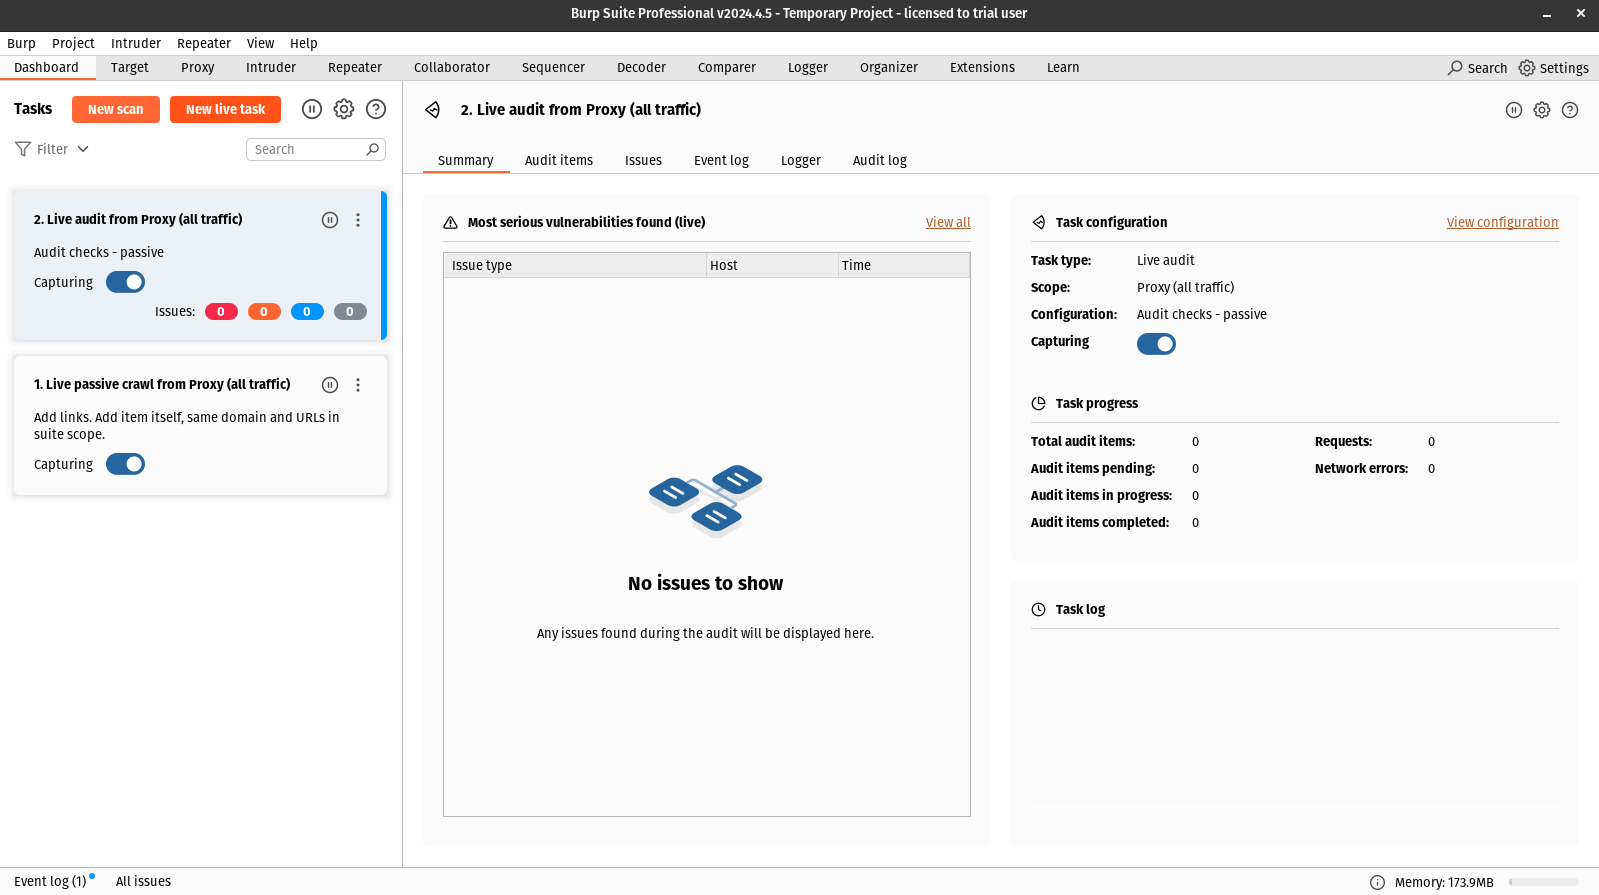
\includegraphics[width=1\textwidth]{slike/burp_start.png}
    \caption{Izgled Burp suita pri pokretanju}
    \label{slk:burp_start}
\end{figure}
\subsection{\textit{Proxy}}
Burp \textit{Proxy} je jedan od glavnih modula Burp Suitea. On omogućava presretanje, pregled i promjenu HTTP i HTTPS zahtjeva između preglednika i web aplikacije. 
Koristeći Proxy, sigurnosni stručnjaci mogu analizirati zahtjeve i odgovore, tražiti ranjivosti i manipulirati podacima kako bi testirali sigurnost web aplikacije.\cite{burp_feat}

\subsection{\textit{Intruder}}
Burp \textit{Intruder} je modul za automatizirane napade. Može se koristiti za \textit{brute force} napade, testiranje valjanosti unosa, traženje skrivenih direktorija ili datoteka, 
te druge vrste napada. Korisnik može konfigurirati različite parametre i payload-ove koji će se automatski slati, a Intruder će analizirati odgovore kako bi identificirao 
potencijalne ranjivosti.\cite{burp_feat}

\subsection{\textit{Repeater}}
\textit{Repeater} omogućava korisnicima da ponavljaju HTTP/HTTPS zahtjeve ručno. Ovo je korisno za detaljno testiranje specifičnih zahtjeva i odgovora. Korisnik može modificirati i 
ponovo poslati zahtjeve, te analizirati odgovore kako bi identificirao ranjivosti i prijetnje.\cite{burp_feat}

\subsection{\textit{Collaborator}}
\textit{Collaborator} je modul za otkrivanje server-side ranjivosti koje zahtijevaju interakciju s vanjskim sustavima/stranicama. Primjeri ovih ranjivosti uključuju 
SSRF (engl. \textit{Server-Side Request Forgery}) i različite vrste injekcija koje rezultiraju vanjskim interakcijama. Omogućava postavljanje posebnog servera koji prati 
ove interakcije i pomaže u identifikaciji ranjivosti.\cite{burp_feat}

\subsection{\textit{Comparer}}
\textit{Comparer} omogućava uspoređivanje dva skupa podataka. Ovo može biti korisno za analizu promjena između dva odgovora ili zahtjeva, kako bi se identificirale suptilne razlike koje 
mogu ukazivati na ranjivosti kao što su neodgovorna obrada zahtjeva pri kojoj mogu iscuriti informacije iz takozvanih 'sporednih kanala'. \cite{burp_feat}

\subsection{\textit{Extensions}}
\textit{Extensions} modul omogućava proširivanje funkcionalnosti Burp Suitea putem dodataka (ekstenzija). Korisnici mogu instalirati ekstenzije iz BApp Storea ili kreirati 
vlastite koristeći Burp Extender API. Ovo omogućava prilagođavanje alata specifičnim potrebama i dodavanje novih funkcija koje nisu dostupne u osnovnoj verziji.\cite{burp_feat}


\newpage
\section{Usporedba alata \textit{a priori}}
U svojoj suštini ZAP i Burp suite Professional imaju iste funkcionalnosti. Kroz godine su OWASP i nezavisni programeri polako gradili alat koji sada već može parirati profesionalnom
plaćenom alatu.
Kao što se iz tablice \ref{tbl:usporedba} zaključiti ZAP po svemu parira Burp suite-u, no i dalje oba alata imaju prednosti i mana. Jedna od većih mana Burp Professional Suita je njegova cijena gdje će nas samo jedna godina licence koštati 450 eura.
Manjkavost ZAP-a je \textit{Fuzzer}. U trenutku izrade rada funkcionalnost tog modula nije u potpunosti realizirana kao kod Burp-a što će kasnije biti pokazano.
Funkcionalnosti koje ZAP ima a Burp suite nema su mogućnost automatizacije i HUD (engl. \textit{Heads Up Display}). Automatizaciju ZAP sam prije spomenuo a HUD ću koristiti i objasniti prilikom testiranja.
Što se tiče korisničkog sučelja oba alata pružaju lijepo i moderno sučelja, gdje Burp ima malu prednost zbog jasnoće i intuitivnosti kartica i modula.
\begin{table}[H]
  \centering
  \caption{Burp suite modul i odgovarajuća alternativa realizirana u ZAP-u\cite{burp_to_zap}}
  \begin{tabular}{|c|c|}
      \hline
      \textbf{Burp Suite Professional značajka} & \textbf{ZAP alternativa} \\
      \hline
      Collaborator & OAST Support Add-on \\
      Comparer & Diff \\
      Decoder & Encoder \\
      DOM Invader & Eval Villian ekstenzija \\
      Extender & Marketplace, Scripts \\
      Intercept & Breakpoints \\
      Intruder & Fuzzer\textbf{*} \\
      Live scan & ATTACK Mode \\
      Project Files & Session Files \\
      Proxy & Proxy \\
      Repeater & Manual Request Editor, Requester ekstenzija \\
      Scanner & Active Scanner \\
      Sequencer & Token Generation and Analysis \\
      Target & Contexts \\
      \hline
  \end{tabular}
\label{tbl:usporedba}
\end{table}
% \chapter{Testiranje}
%\section{Opis testiranja}
Jedini pravi način da se objektivno usporedi efektivnost oba alata jest da ih se testira na realnim i konkretnim situacijama. Za testiranje će se koristiti Burp Suite Web Security Academy laboratorijske vježbe.\cite{burp_labs}
Osim što postoje vodiči za Burp Suite postoje i vodiči za ZAP koje su korisnici pisali.\cite{owasp_2fa_manual,owasp_b-f_manual}
Vježbe su odabrane uz pomoć OWASP Top 10 stranice\cite{owasp_top10} koja vodi brigu o broju i vrsti sigurnosnih rizika koji su do godine pisanja bili najčešći, 
te njihove povezane CWE-ove.
Obraditi će se laboratorijske vježbe povezane sa sigurnosnim rizicima s vrha gore navedenog popisa. Specifično su izabrane one za koje postoje rješenja u ZAP vodiču ili čija se rješenja mogu lako pronaći.
%%%%%%%%%%%%%%%%%%%%%%%%%%%%%%%%%%%%%%%%%%%%%%%%%%%%%%%%%%%%%%%%%%%%%%%%%%%%%%%%%%%%%%%%
%     SQL
%%%%%%%%%%%%%%%%%%%%%%%%%%%%%%%%%%%%%%%%%%%%%%%%%%%%%%%%%%%%%%%%%%%%%%%%%%%%%%%%%%%%%%%%
\section{Vidljiva pogreška bazirana na SQL injekciji}
%\subsection{Općenito}
SQL injekcije su među najčešćim prijetnjama na Internetu. Činjenica koje to dokazuje je da su s ostalim vrstama injekcija 2017.\ predstavljale najrasprostranjeniji sigurnosni rizik ,a 2021.\ su bile čak 
na trećem mjestu po učestalosti.\cite{owasp_top10}
SQL injekcija je tehnika napada u kojoj napadač ubacuje zlonamjerni SQL kod u polja za unos aplikacije kako bi izvršio neovlaštene radnje na bazi podataka. To 
može uključivati dobivanje osjetljivih podataka, izmjenu podataka, brisanje podataka ili izvođenje administrativnih operacija. 
SQL injekcija nastaje zbog neadekvatnog filtriranja ili validacije korisničkog unosa.\cite{clarke_sql,sql_w3}

Laboratorijska vježba sadrži ranjivost na SQL injekcije koju će biti iskorištena. Od ostalih informacija znamo da aplikacija koristi 'kolačiće' za analitiku te provodi SQL upit 
s informacijama u podnesenim kolačićima. Rezultati SQL se ne vraćaju direktno već je potrebno izazvati grešku u ispisu. Baza podataka sadrži tablicu zvanu \textit{users} sa stupcima \textit{username} i \textit{password}.
Cilj laboratorijske vježbe je pronalazak načina da web aplikaciji 'iscuri' lozinka za korisnika \textit{administrator} te se onda treba ulogirati s njihovim računom.

Ono što je također bitno za primjetiti je da se ne koriste podatci dobivene direktno iz malicioznog SQL upita, već grešku koja se zbog upita vraća. To uvelike otežava alatima da primjete takve ranjivosti kako \textit{de facto} nema polja koje bi mogli iskoristiti da nam aplikacija da neke djelove baze podataka direktno. 
Umjesto toga cilj je iskoristiti lošu obradu grešaka.\cite{sql_lab} 

\subsection{Vježba 1: Burp Suite}
Nakon otvaranja alata potrebno je kliknuti na karticu \textit{Target} kako je prikazano na slici \ref{slk:target_burp}.
\begin{figure}[H]
    \centering
    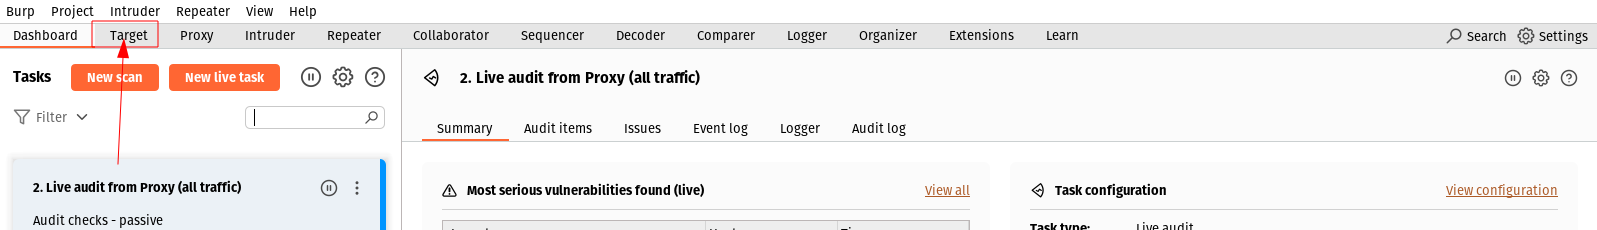
\includegraphics[width=1\textwidth]{slike/BURP_target.png}
    \caption{Popis svih kartica s naznačenom karticom \textit{Target}}
    \label{slk:target_burp}
\end{figure}

Ondje je prije svega potrebno uključiti proxy koji će biti korišten za presretanje zahtjeva i odgovora. Zatim je potrebno kliknuti na gumb \textit{Open browser} te u adresnu traku zalijepiti adresu laboratorijske
vježbe. Odmah prilikom otvaranja dediciranog pretraživača i unosom poveznice na vježbu Burp izgradi \textit{sitemap} (mapu cijele stranice).
Sada kako bi bilo moguće pronaći ranjivost koja će se iskoristiti za navedenu vježbu nužno je započeti skeniranje s kartice \textit{Dashboard > New scan > Webapp scan}.
Najprije se prikazuje pregled skena kao što je vidljivo na slici \ref{slk:burp_pojed}. Ovdje se mogu vidjeti generalne informacije o meti i trenutnim postavkama skena.
Potom se konfigurira sken kao što je to vidljivo na slici \ref{slk:burp_config}. Prilikom ove i budućih vježbi koristiti će se \textit{Deep} sken.
\begin{figure}[H]
    \centering
    \begin{minipage}[b]{0.46\textwidth}
      \centering
      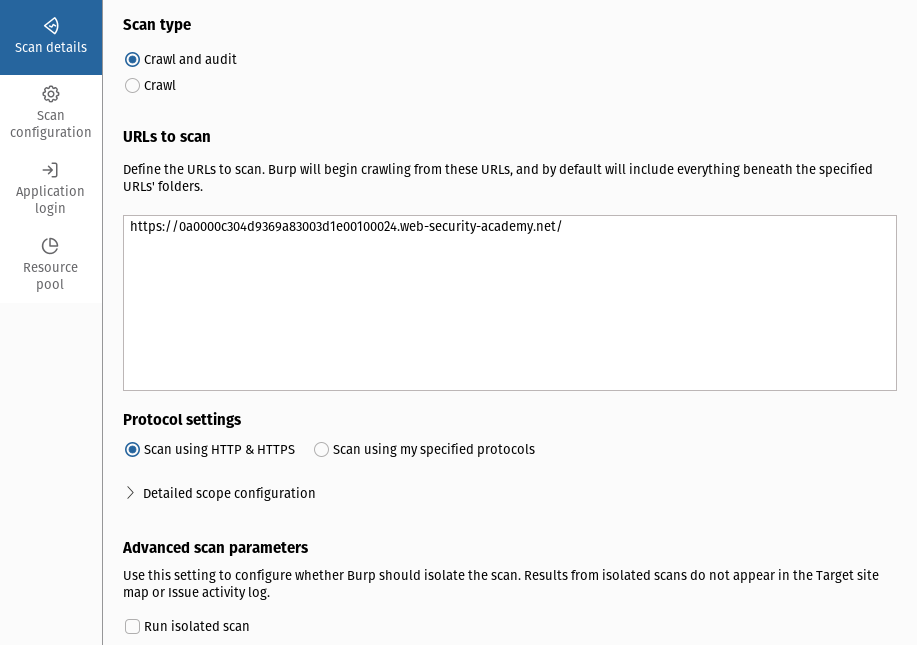
\includegraphics[width=\textwidth]{slike/scan_det.png}
      \caption{Pojedinosti skena}
      \label{slk:burp_pojed}
    \end{minipage}
    \hspace{0.05\textwidth} % Razmak između slika
    \begin{minipage}[b]{0.47\textwidth}
      \centering
      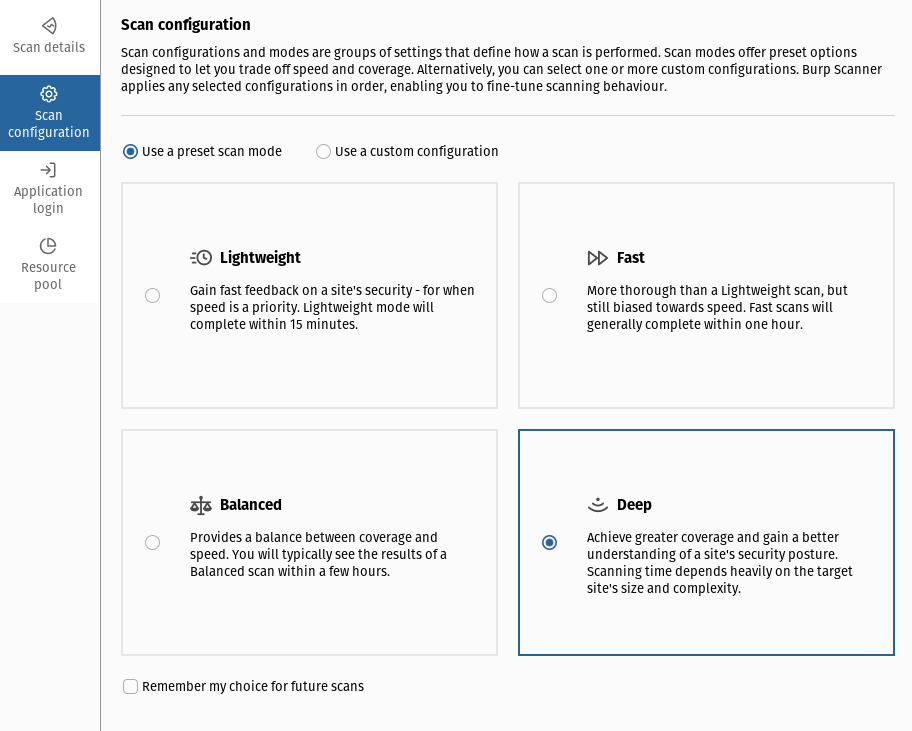
\includegraphics[width=\textwidth]{slike/scan_config_burp.png}
      \caption{Konfiguriranje skena}
      \label{slk:burp_config}
    \end{minipage}
  \end{figure}

\lstset{language=SQL}
Skeniranje traje <5 minuta te izvodi očekivane rezultate. Osim SQL ranjivosti, alat je pronašao nekolicinu informativnih detalja što se stranice tiče poput činjenice da komunikacija nije enkriptirana 
te kako nije definirana striktna sigurnosna politika za transport.
Vezano za SQL injection alat je pronašao ranjivosti na čak 3 putanje \textit{/product, /filter} i \textit{/my-account}. Za product i filter je koristio \textit{payload} u kojem je u
\textit{trackingid} prvo dodao jednu ' a nakon što je aplikacija javila grešku dodao '' na kraj \textit{TrackingId}-a nakon koje je greška nestala. Zatim je pokušao napraviti novi payload viljiv na slici \ref{slk:burp_auto}
nakon čega je primijetio da stranici treba dulje da odgovori te je deducirao da se najvjerojatnije radi o Postgres bazi podataka. Sa slike je vidljivo kako je iskorištena naredba za spavanje integrirana kao dio \textit{TrackingId}-a koju 
baza nakon parsiranja izvršava.

\begin{figure}[h]
  \centering
  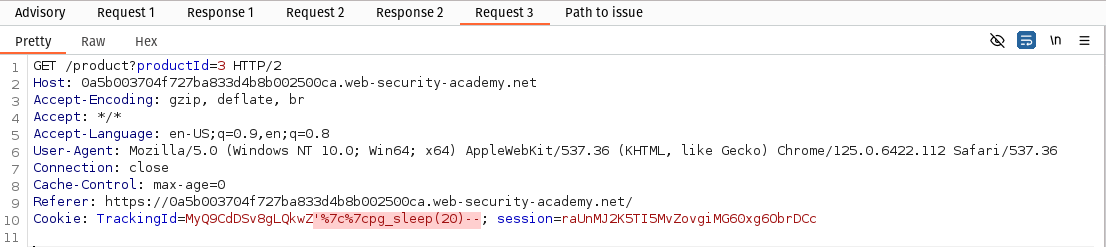
\includegraphics[width=1\textwidth]{slike/sql_requests.png}
  \caption{Zahtjev koji je otkrio bazu podataka i iskoristio SQL ranjivost}
  \label{slk:burp_auto}
\end{figure}

Pod karticom \textit{Advisory} s slike \ref{slk:burp_auto} je vidjljivo koji CWE se krije iza otkrivene ranjivosti te detalje o ispitanoj ranjivosti. Sada je potrebno iskoristiti ovo znanje prilikom napada web aplikacije te potom izvršiti prijavu kao \textit{administrator}.
Prvo se navigira u karticu \textit{Proxy > HTTP history}. Ondje se nalazi GET zahtjev za putanju \textit{/login} te je potrebno modificirati dio kolačića gdje piše \textit{TrackingId} tako da na kraj vrijednosti stoji '.
To će natjerati stranicu da izbaci pogrešku iz kojeg se otkriva cijeli SQL upit što je vidljivo na slici \ref{slk:err_test}.

\begin{figure}[]
    \begin{lstlisting}[frame=single, breaklines]
        Unterminated string literal started at position 52 in SQL SELECT * FROM tracking WHERE id = 'JhlbaDuQVof0JeOw''. Expected char
    \end{lstlisting}
    \caption{Dobivena pogreška}
    \label{slk:err_test}
\end{figure}

Sada je potrebno modificirati taj zahtjev kako bi došli do lozinke korisnika \textit{administrator}. Dobar bi pokušaj bio potpuno maknuti vrijednost \textit{TrackingId} argumenta i zamijeniti ju sa zloćudnim SQL upitom.
Koristeći Repeater modul (desni klik na zahtjev > \textit{Send to Repeater}) te ćemo ondje izmijeniti vrijednost tako da sad u payload-u piše: \newline
\textit{TrackingId=' AND 1=CAST((SELECT username FROM users LIMIT 1) AS int)--}

Iz prijašnje greške \ref{slk:err_test} može se zaključiti da aplikacija traži samo jedan \textit{TrackingId} te da je vjerojatno potrebno ograničiti upit na jedan redak baze kao i jedan stupac.
Sada bi trebala doći nova greška koja kaže kako \textit{administrator} nije tipa \textit{integer}. Iz ove greške je očito da se administrator nalazi prvi na popisu. Kao što je vidljivo potrebno je pretvoriti polja koja nisu \textit{integeri} u \textit{int} upravo kako bi 
natjerali bazu da "procuri informacije".
Ponovno ćemo se sada vratiti u \textit{Repeater} te ponoviti prijašnji zahtjev s malom preinakom:\newline
\textit{TrackingId=' AND 1=CAST((SELECT password FROM users LIMIT 1) AS int)--}

Ovaj upit napokon otkriva password za korisnika \textit{administrator} \ref{slk:err_good} no kao grešku.
\begin{figure}[H]
    \begin{lstlisting}[frame=single, breaklines]
        ERROR: invalid input syntax for type integer: "vuapcoxchp374pzq5d31"
    \end{lstlisting}
    \caption{Pogreška koja ispisuje lozinku za administratora}
    \label{slk:err_good}
\end{figure}
\newpage % dodano radi urednosti
\subsection{Vježba 1: ZAP}
Najprije u gornjem desnom kutu alat je potrebno postaviti \textit{Mode} na ATTACK. Zatim je potrebno kliknuti na \textit{Automated scan} i unijeti link mete.
Skeniranje traje nešto dulje od Burpovog. Među alertima je vidljivo da ZAP nije primijetio da uopće postoji mogućnost SQL injection-a\ref{slk:zap_vuln}. Prije je spomenuto kako ZAP ima Fuzzer ali nije trenutno funkcionalan. Razlog tomu je što ZAP trenutno nema mogućnost 
skeniranja HTTP zaglavlja što je veliki minus u odnosu na Burp.\cite{burp_to_zap} Ovaj zadatak služi otkrivanju ove velike manjkavosti ZAP-a nad Burpom.
\begin{figure}[H]
    \centering
    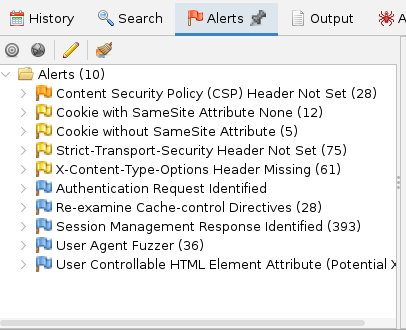
\includegraphics[width=0.8\textwidth]{slike/zap_sql_alerts.png}
    \caption{Manjak upozorenja na ranjivosti web aplikacije}
    \label{slk:zap_vuln}
\end{figure}

Problem je moguće zaobići koristeći ZAP HUD.\@ To je modul koji omogućava ručnu provjeru, izmjenu i slanje zahtjeva. Nakon što se uključi \textit{Break} prilikom gledanja \textit{/login} putanje nakon klika na gumb Login.
Ovdje je potrebno izmijeniti HTTP zaglavlje te modificirati kolačić kao što je prethodno to učinjeno za Burp. Naravno sada je otkriveno dobro rješenje na isti način kao i za Burp.
%%%%%%%%%%%%%%%%%%%%%%%%%%%%%%%%%%%%%%%%%%%%%%%%%%%%%%%%%%%%%%%%%%%%%%%%%%%%%%%%%%%%%%%%
%     2FA
%%%%%%%%%%%%%%%%%%%%%%%%%%%%%%%%%%%%%%%%%%%%%%%%%%%%%%%%%%%%%%%%%%%%%%%%%%%%%%%%%%%%%%%%
\newpage % dodano radi urednosti
\section{Dvofaktorska autentifikacija sa pogrešno konfiguriranom logikom}
%\subsection{Općenito}
Dvofaktorska autentifikacija (2FA) je sigurnosni mehanizam koji koristi dva različita faktora za provjeru identiteta korisnika, kao što 
su lozinka (prvi faktor) i jednokratni kod poslan putem SMS-a ili aplikacije (drugi faktor). Iako 2FA značajno povećava sigurnost, može 
biti ranjiv na određene vrste napada ako nije pravilno implementiran.\cite{dmitrienko2014security,aloul2009two}
Primjeri loše implementacije su recikliranje sigurnosnih kodova, realizacija 2FA na klijentskoj strani, direktan pristup API-ju, loša programska potpora i mnogi drugi.

Ova laboratorijska vježba ima ranjivost u dvofaktorskoj autentifikaciji zbog pogrešne logike, konkretno uz zahtjev za unos sigurnosnog koda u kolačiću prenosi i ime korisnika te nema limit na slanje zahtjeva što uvelike kompromitira aplikaciju.
Za rješavanje zadataka, potrebno je pristupiti računu korisnika \textit{Carlosa}.
Kao informacije za vježbu su pruženi podatci za pristup korisniku \textit{wiener} s lozinkom \textit{peter} te pristup mail serveru.\cite{2FA_lab}
Također je dan hint kako se korisnik \textit{carlos} neće pokušati ulogirati za vrijeme trajanja napada.

\subsection{Testiranje: Burp Suite}
Skeniranje se pokreće kao u prethodnoj vježbi. 
Kao u stvarnim situacijama, zanimljivi su POST zahtjevi koje skener šalje. 
Pokušat će se iskoristiti \textit{/login} putanja za rješavanje vježbe. 
Prije svega, pokušava se ulogirati s danim vjerodajnicama, nakon čega se traži unos 4-znamenkastog koda koji je poslan na mail. 
Već sada se uočava manjkavost realizacije. 
Ako kod ima samo 4 znamenke, to znači da postoji samo 10,000 mogućih kombinacija što nije puno za današnje sustave. 
Nakon što se uspije, pretražit će se povijest skeniranja da se vidi kako se zahtjev može izmijeniti.

Zahtjev sa putanjom \textit{/login2} šalje se na \textit{Intruder} kao što je vidljivo na slici \ref{slk:burp_req}. 
Jednom kada se uđe u Intruder, vrijednost \textit{verify} iz \textit{wiener} mijenja se u \textit{carlos} za GET zahtjev, što generira privremeni kod. 
Zatim se POST zahtjev iste putanje šalje na Intruder te se bira način rada \textit{Sniper} i označava vrijednost polja \textit{mfa-code} za modificirani payload što je vidljivo na \ref{slk:burp_req_config}. 
Burp će sada slati zahtjeve, svaki put modificirajući payload, kako bi pogodio točan kod za carlosa.

\begin{figure}[H]
  \centering
  \begin{minipage}[b]{0.45\textwidth}
    \centering
    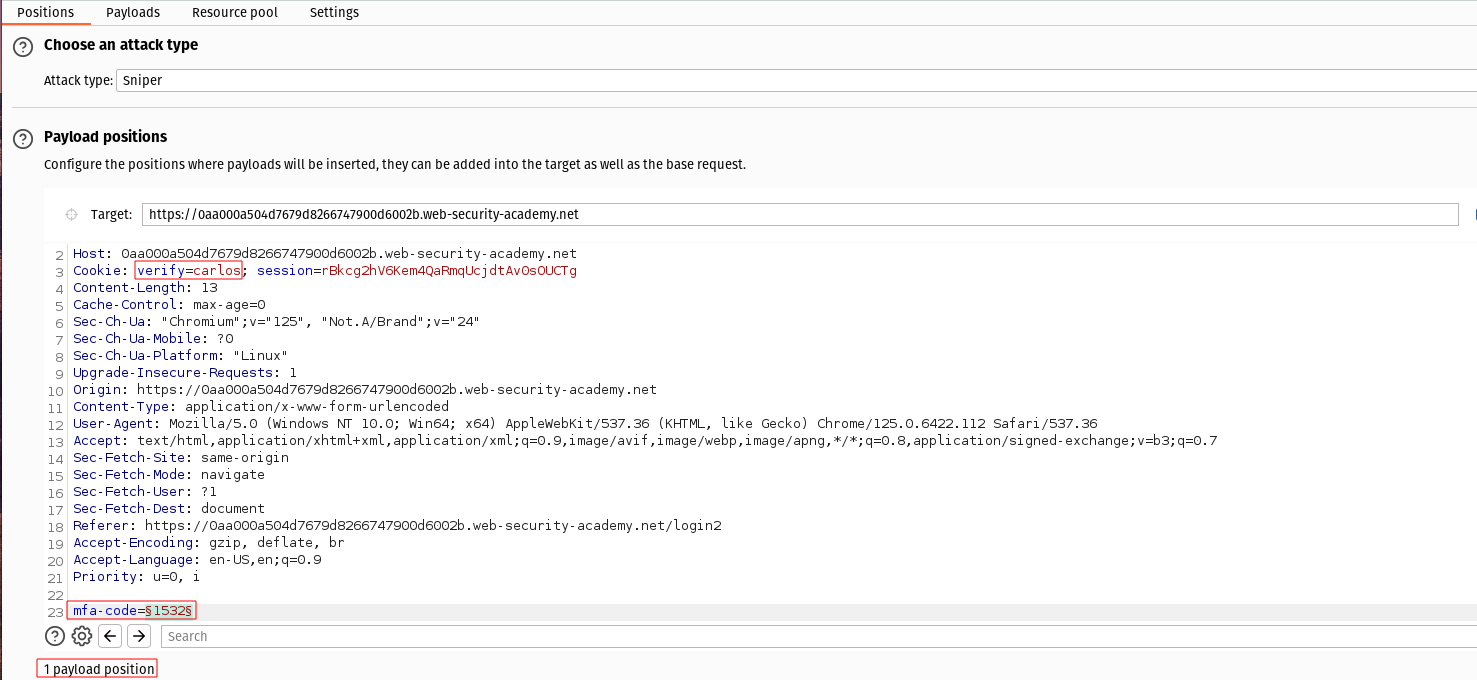
\includegraphics[width=\textwidth]{slike/intruder_2fa.png}
    \caption{Zahtjev koji ćemo koristiti u Intruderu}
    \label{slk:burp_req}
  \end{minipage}
  \hspace{0.05\textwidth} % Razmak između slika
  \begin{minipage}[b]{0.45\textwidth}
    \centering
    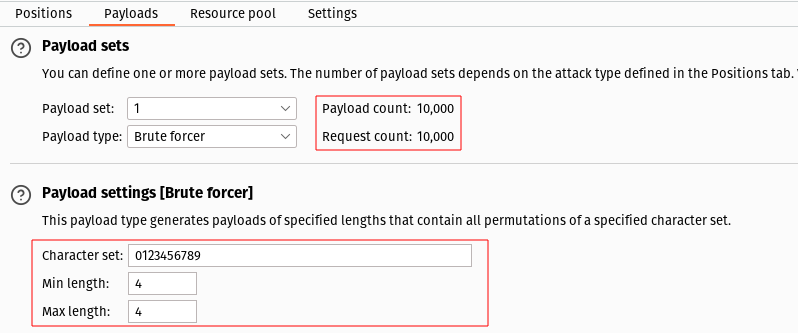
\includegraphics[width=\textwidth]{slike/payload_intruder.png}
    \caption{Konfiguriranje payloada}
  \end{minipage}
  \label{slk:burp_req_config}
\end{figure}

Sada se traži odgovor koji se razlikuje od drugih ili po duljini ili po vrsti odgovora. U ovom slučaju razlikovat će se i po vrsti i po duljini odgovora\ref{slk:burp_atks}. Jedan jedini payload vratio se s odgovorom 302, što označava redirekciju. Kada se pogleda vrijednost payloada za taj zahtjev, vidi se da je Carlosov trenutačni kod 0100.
\begin{figure}[H]
  \centering
  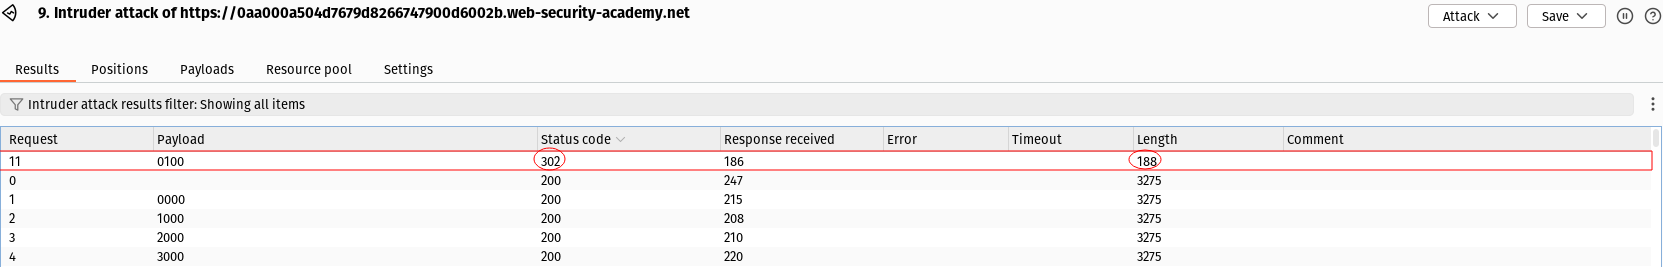
\includegraphics[width=1\textwidth]{slike/intruder_atk.png}
  \caption{Prikaz napada uz modul Intruder}
  \label{slk:burp_atks}
\end{figure}

Odgovor se učita u pretraživač ili se kod ručno unese, čime se završava vježba. Pritom se mora paziti da se na preostalim zahtjevima za vrijednost \textit{verify} upiše \textit{carlos}.\newpage % dodano radi urednosti

\subsection{Testiranje: ZAP}
Kako je već mnogo poznato o web aplikaciji, testiranje se može brže provesti. Sa ZAP HUD-om se ponovno normalno ulogira kao što je to učinjeno kod Burpa. Nakon što se ulogira s danim vjerodajnicama, otići će se u karticu \textit{History} u glavnom izborniku. Ondje se izabire GET zahtjev za \textit{/login2} putanju, te mu se modificira vrijednost \textit{verify} i zahtjev se šalje.

Zatim se pronađe stari POST zahtjev za \textit{/login2}. Kako generator regularnih izraza nije funkcionalan u ZAP-u, potrebno je napraviti kratki "obilazak". Prvo se dodaje generator zahtjeva tipa \textit{Numberzz}, koji stvara brojeve od 0 do 9999 što je vidljivo na slici \ref{slk:zap_gen}. Nakon toga je iz slike \ref{slk:zap_config_proc} vidljivo da je potrebno namjestiti procesor za zahtjeve koji će zahtjeve pretvoriti u oblik koji je zapravo potreban.
\begin{figure}[H]
  \centering
  \begin{minipage}[b]{0.5\textwidth}
    \centering
    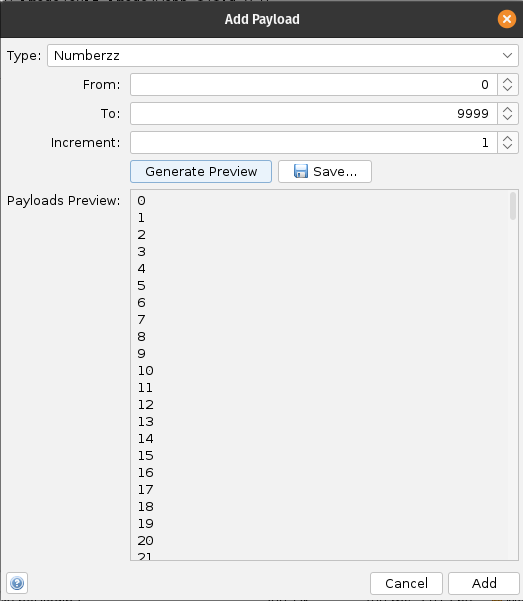
\includegraphics[width=\textwidth]{slike/payload_fuzz.png}
    \caption{Dodavanje generatora}
    \label{slk:zap_gen}
  \end{minipage}
  \hspace{0.05\textwidth} % Razmak između slika
  \begin{minipage}[b]{0.4\textwidth}
    \centering
    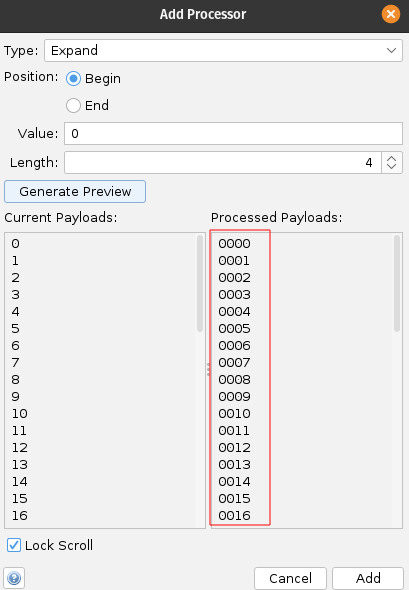
\includegraphics[width=\textwidth]{slike/processor_fuzz.png}
    \caption{Konfiguriranje procesora zahtjeva}
    \label{slk:zap_config_proc}
  \end{minipage}
\end{figure}

Kao i u radu s Burpom sada se pronalazi odgovor koji se razlikuje te se šalje pregledniku. Nakon toga bi se trebalo pojaviti na zaslonu nešto kao na slici \ref{slk:zap_succ}.

\begin{figure}[H]
  \centering
  
\includegraphics[width=0.4\textwidth]{slike/2fa_succ.png}
  \caption{Prikaz uspješne prijave}
  \label{slk:zap_succ}
\end{figure}
%%%%%%%%%%%%%%%%%%%%%%%%%%%%%%%%%%%%%%%%%%%%%%%%%%%%%%%%%%%%%%%%%%%%%%%%%%%%%%%%%%%%%%%%
%     Brute force
%%%%%%%%%%%%%%%%%%%%%%%%%%%%%%%%%%%%%%%%%%%%%%%%%%%%%%%%%%%%%%%%%%%%%%%%%%%%%%%%%%%%%%%%
\section{Napad silom na lozinku koristeći lošu implementaciju promjene lozinke}
Napad grubom silom na lozinku podrazumijeva isprobavanje svih mogućih kombinacija dok se ne pronađe točna. 
Kada se kombinira s loše implementiranom funkcionalnošću promjene lozinke, mogu se pojaviti ozbiljni sigurnosni problemi. 
Primjerice, ako sustav dopušta korisniku da promijeni lozinku bez provjere identiteta putem adekvatnih metoda (npr. slanje privremene lozinke na unaprijed spremljeni mail, korištenje dvofaktorske autentifikacije), otvara se prostor za iskorištavanje ranjivosti.
U takvim scenarijima, napadač koji dobije pristup korisničkom računu putem metoda poput napada grubom silom ili socijalnog inženjeringa može lako promijeniti lozinku i time zaključati legitimnog korisnika. 
To se događa jer sustav ne provjerava dovoljno identitet korisnika prije nego što dopusti promjenu lozinke.

Kako bi se smanjili rizici, ključno je implementirati robustne sigurnosne mjere poput dvofaktorske autentifikacije, obavijesti o promjeni lozinke na registrirani virtualni sandučić (engl. \textit{mail}), specifične fraze koje se generiraju za svakog korisnika pri registraciji i slična rješenja.
Nažalost, napade grubom silom je gotovo nemoguće spriječiti te bi dizajneri trebali ciljati na to da je ovo najbolji mogući napad koji se pruža napadačima jer je ekstenzivan te u puno slučajeva zahtjeva puno vremena i resursa.\cite{knudsen2011brute} 

Sigurnosni propust u funkcionalnosti promjene lozinke u ovoj laboratorijskoj vježbi čini ju podložnom napadima grubom silom. Za rješavanje ove vježbe, potrebno je iskoristiti listu potencijalnih lozinki kako bi se pristupilo Carlosovom korisničkom računu. 
Informacije koje su na raspolaganju uključuju vlastite vjerodajnice (wiener:peter), korisničko ime \textit{carlos}, te listu kandidata za lozinku u obliku teksta gdje je svaka potencijalna lozinka zapisana u zaseban redak.\cite{brute_lab}
\newpage %dodano radi preglednosti
\subsection{Testiranje: ZAP}
Prije nego što se započne s ručnim testiranjem aplikacije, provest će se automatizirani sken kako bi se dobila mapa povezanih stranica (engl. \textit{sitemap}). 
Iako neće puno pomoći u rješavanju ove konkretne vježbe, uvijek je dobra praksa ispitati površinu napada kako bi se mogao pronaći dobar vektor napada. 
Sken sam po sebi ne otkriva previše, tako da će se pristupiti ručnom testiranju aplikacije uz pomoć ZAP HUD-a.

Prva stvar koja će se napraviti je prijava s danim vjerodajnicama kako bi se vidjelo kako aplikacija gradi zahtjeve za prijavu. 
Za to će poslužiti modul \textit{Break}, koji omogućuje pregled i uređivanje svakog zahtjeva prije nego što ga preglednik pošalje i odgovora prije nego što ga preglednik primi. 
Iako naslov vježbe sugerira da vjerojatno neće biti moguće iskoristiti funkcionalnost prijave, dobro je biti temeljit i vidjeti postoji li neka ranjivost koja nije namjerno ostavljena. 
U ovom konkretnom slučaju, prijava je dobro implementirana, te će se nastaviti s testiranjem. 
Sada je zaslon nakon prijave nešto drukčiji nego na prijašnjim vježbama kao što je vidljivo na slici \ref{slk:succ_login}. Vidljivo je da je osim unosa maila moguća i promjena lozinke ukoliko je poznata trenutna.
\begin{figure}[H]
  \centering
  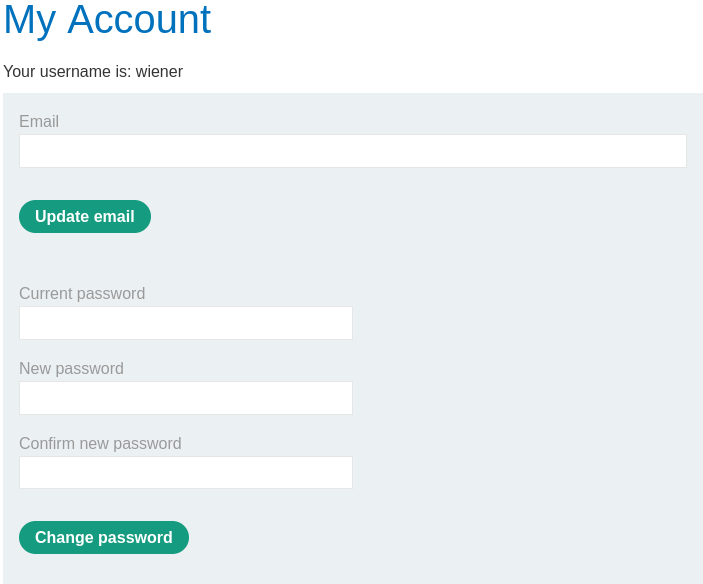
\includegraphics[width=0.6\textwidth]{slike/b_f_postLogin.png}
  \caption{Sučelje nakon prijave sa dostupnim vjerodajnicama}
  \label{slk:succ_login}
\end{figure}

Očito je da se mora dokučiti kako iskoristiti opcije za mijenjanje lozinke. 
Pokušat će se promijeniti lozinka računu kojem se ima pristup kako bi se vidjelo kako web aplikacija gradi zahtjev. 
Ponovno će se koristiti \textit{Break} funkcionalnost kako bi se presreo i uredio zahtjev vidljiv na slici \ref{slk:gen_req}. 
Označeno je tijelo zahtjeva koje je potrebno urediti.

\begin{figure}[H]
  \centering
  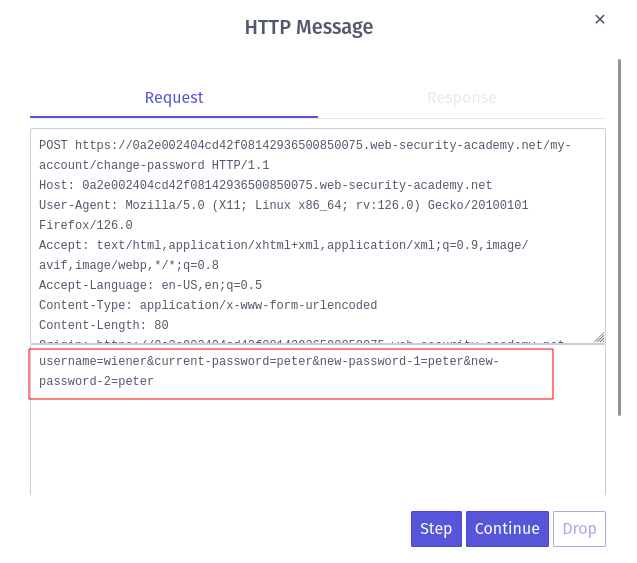
\includegraphics[width=0.8\textwidth]{slike/break_np.png}
  \caption{Zahtjev koji aplikacija generira}
  \label{slk:gen_req}
\end{figure}

Iz slike \ref{slk:gen_req} je vidljivo da se, kao u prijašnjim vježbama, može mijenjati korisničko ime kao i pripadajuća lozinka. 
Sada, kada su te putanje spremljene, koristit će se \textit{Fuzzer} kako bi se razotkrila lozinka za korisnika \textit{carlos}. 
Kako izmjena lozinki zapravo nije moguća, potrebno je na drugi način dokučiti koja je lozinka točna.
Relevantni POST zahtjev šalje se u \textit{Fuzzer}. 
Unutar \textit{Fuzzer}a korisničko ime \textit{wiener} zamjenjuje se s \textit{carlos}, a trenutna lozinka označava se kao mjesto na kojem će alat pogađati lozinke. 
Također, alat se opskrbljuje kandidatima za lozinku koji su dobiveni na početku vježbe, te se postavljaju različite nove lozinke. 
To se radi kako bi se umjesto pogreške da je lozinka netočna dobio odgovor koji javlja da se nove lozinke ne poklapaju. 
Primjer tako definiranog zahtjeva možemo vidjeti na slici \ref{slk:full_config_fuzz_zap}

\begin{figure}[H]
  \centering
  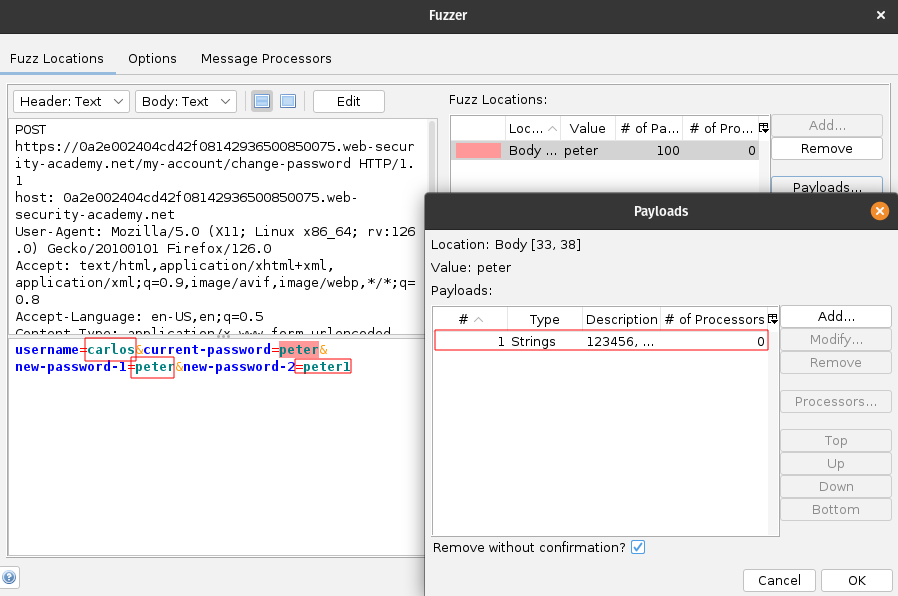
\includegraphics[width=1\textwidth]{slike/zap_fuzz_pass.png}
  \caption{Ispravno konfiguriran \textit{Fuzzer}}
  \label{slk:full_config_fuzz_zap}
\end{figure}

Sada se traži odgovor koji, među onima kojima su zaprimljeni ima različitu duljinu odgovora. 
Uz njega nam piše i koju je lozinku alat pokušao poslati. 
Sada je potrebno tu lozinku iskoristiti da za prijavu kao \textit{carlos} i tako završava ova laboratorijska vježba.

\newpage %dodano radi preglednosti
\subsection{Testiranje: Burp Suite}
Kao i za ZAP, aplikacija će se prvo skenirati kako bi se utvrdila površina napada. 
Kao i kod ZAP-a, skener nije utvrdio nikakve probleme. 
Unese se ispravna trenutna lozinka i dvije nove lozinke koje se ne podudaraju. 
Ovaj zahtjev POST /my-account/change-password šalje se u Burp Intruderu. 
Zbog prijašnjeg testiranja, zna se da je potrebno pratiti razlike u odgovorima.
U Burp Intruderu parametar username mijenja se u carlos i dodaje se položaj za promjenu za parametar trenutne lozinke. 
Provjerava se da su parametri za nove lozinke postavljeni na dvije različite vrijednosti. 
Na kartici \textit{Payloads} unosi se lista lozinki.
Kada je napad završen, može se primijetiti da je jedan odgovor drukčije duljine i sadrži poruku "Nove lozinke se ne podudaraju". 
Lozinka koja je iskorištena u tom zahtjevu je lozinka za račun \textit{carlos} što je vidljivo na slici \ref{slk:atk_end}.

\begin{figure}[H]
  \centering
  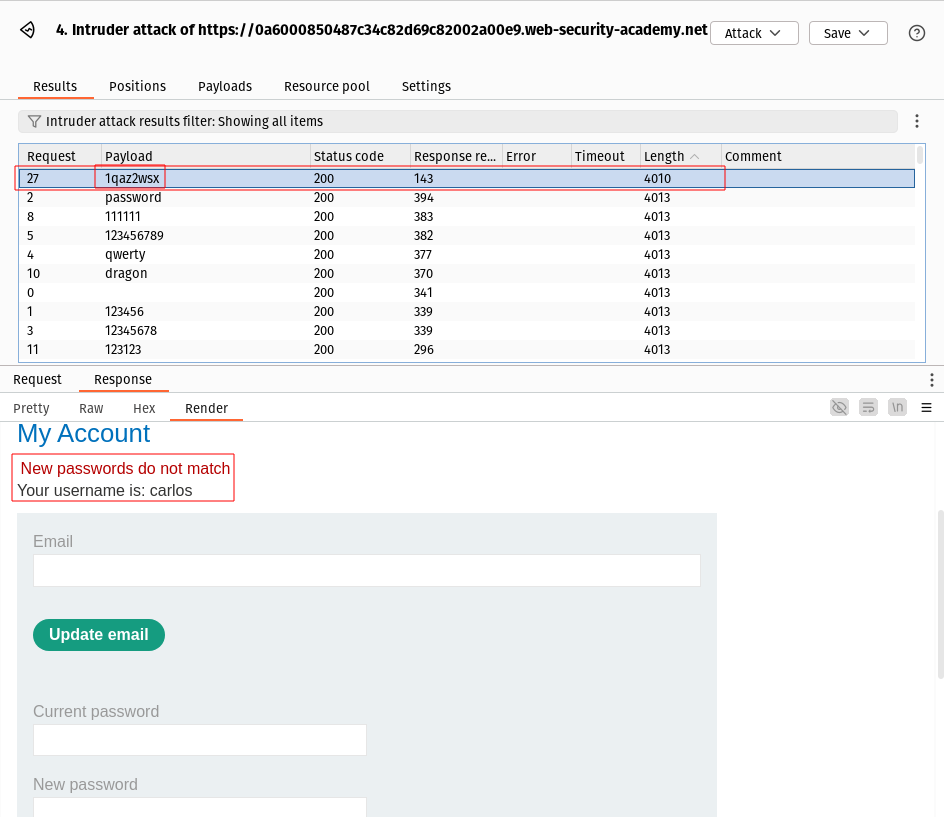
\includegraphics[width=1\textwidth]{slike/butp_bf_fuzz.png}
  \caption{Kraj napada u \textit{Intruder}u}
  \label{slk:atk_end}
\end{figure}
Rješenje u ovom slučaju je \textbf{1qaz2wsx} što je i vidljivo iz slike \ref{slk:atk_end}.
% \chapter{Usporedba i nadomještanje funkcionalnosti}
%\addcontentsline{toc}{chapter}{Usporedba i nadomještanje funkcionalnosti}
Oba alata imaju slične funkcionalnosti i mogu postići iste rezultate s minimalno različitim pristupom. 
ZAP je očito namijenjen za male tvrtke i pojedince, dok je Burp Suite komercijalan alat namijenjen za velike tvrtke i korporacije. 
Iako i velike tvrtke mogu koristiti ZAP, njihovi sigurnosni specijalisti moraju proći više obuke.

Razlike u korištenju su primijećene prilikom korištenja oba alata. 
Kada se pojavi problem s Burpom ili je potrebna informacija o njihovim alatima, uvijek se može osloniti na dobro napisanu dokumentaciju. 
\textit{PortSwigger} (tvrtka koja je izgradila Burp Suite) osigurava profesionalne priručnike i video upute za korištenje svojih alata.

Kada se pojavi problem sa ZAP-om, uvelike se oslanja na rješenja koja su već dokumentirali članovi zajednice. 
Iako ZAP ima svoje priručnike i dokumentaciju, oni nisu na razini jasnoće, pokrivenosti i razumljivosti kao Burpova dokumentacija. 
Velika prednost ZAP-a je njegov HUD, koji je bio izuzetno koristan prilikom testiranja. 
U prednost ZAP-u također idu i dodaci, tj. ekstenzije, kojih ima puno više nego za Burp. 
Te ekstenzije mogu se pisati u \textit{Javi, Pythonu, Rubyu, JavaScriptu}, itd. 
Osim toga, ZAP je moguće uključiti u skripte te na taj način automatizirati testiranje.

Primjer takve skripte:

\captionsetup[figure]{labelformat=empty, labelsep=none}

\begin{figure}[H]
    \begin{verbatim}
    import time
    from zapv2 import ZAPv2

    def zap_scan(target_url, api_key='vas_api_kljuc', log='zap_rezultati.txt'):
        zap = ZAPv2(apikey=api_key)
        zap.urlopen(target_url)
        time.sleep(2)
        zap.spider.scan(target_url)
        while int(zap.spider.status('')) < 100:
            time.sleep(2)
        zap.ascan.scan(target_url)
        while int(zap.ascan.status('')) < 100:
            time.sleep(5)
        alerts = zap.core.alerts() # rjecnik alarma
        with open(log, 'w') as f:
            for alert in alerts:
                f.write(f"Alert: {alert['alert']}\nRisk: {alert['risk']}\n \
                URL: {alert['url']}\n Description: {alert['description']}\n \
                Solution: {alert['solution']}\nReference: {alert['reference']}\n)

    if __name__ == "__main__":
        target_url = input("Unesite URL zrtve: ")
        zap_scan(target_url)
    \end{verbatim}
    \captionsetup{labelformat=empty} % To remove the default "Figure" label
    \caption{\textbf{Ispis 3.18.} Jednostavna skripta za automatizaciju skeniranja u Pythonu\cite{zap_script}}
    \label{inp:script}
\end{figure}

Jedino što je potrebno napraviti je instalirati ZAP i Python, postaviti api ključ za korištenje, pokrenuti ZAP u \textit{daemon} načinu rada
te onda sa Pythonovim menadžerom za pakete instalirati paket za korištenje ZAP daemona.

\noindent
\texttt{./zap.sh -daemon -config api.key=your\_api\_key}\newline
\texttt{pip install python-owasp-zap-v2.4}
% \chapter{Zaključak}
Ovaj rad dokazuje da OWASP ZAP može poslužiti kao adekvatna zamjena za Burp Suite Professional u mnogim aspektima 
testiranja sigurnosti web aplikacija. Provedena testiranja na konkretnim laboratorijskim vježbama pokazala su da oba alata mogu 
detektirati i iskoristiti iste ranjivosti, iako ponekad različitim pristupima.
ZAP se istaknuo svojim intuitivnim sučeljem, posebice HUD-om koji olakšava interaktivno testiranje. 
Također, njegova otvorenost za proširenja i mogućnost automatizacije putem skripti čine ga izuzetno fleksibilnim alatom. 
S druge strane, Burp Suite Professional nudi nešto sofisticiraniji skup alata i bolje dokumentiranu podršku, što ga čini preferiranim 
izborom za veće organizacije i profesionalne penetracijske testere.

Ipak, postoje određene funkcionalnosti u kojima ZAP zaostaje, poput nemogućnosti skeniranja HTTP headera, što je bilo vidljivo u vježbi 
s SQL injekcijom. No, takvi nedostaci često se mogu nadomjestiti korištenjem dodataka ili alternativnih metoda.
Ključna prednost ZAP-a je svakako njegova dostupnost kao besplatnog alata otvorenog koda, što ga čini pristupačnim pojedincima i manjim 
timovima koji si ne mogu priuštiti skupe licence. Uz to, aktivna zajednica koja stoji iza ZAP-a kontinuirano radi na poboljšanjima i  
proširenjima, čime se ovaj alat neprestano unapređuje.

Zaključno, iako Burp Suite Professional i dalje drži vodeću poziciju na tržištu, OWASP ZAP se pokazao kao snažan i sposoban alat koji 
može zadovoljiti većinu potreba u području testiranja sigurnosti web aplikacija. Izbor između ova dva alata često će ovisiti o 
specifičnim potrebama projekta, raspoloživom budžetu i stručnosti tima. U svakom slučaju, postojanje kvalitetne besplatne alternative 
poput ZAP-a značajno decentralizira tržište alatima za kibernetičku sigurnost, što u konačnici doprinosi sigurnijem web okruženju te 
osigurava nadmetanje i konstantnu inovaciju.
%\bibliography{literatura}
\chapter{Uvod}
\par Sigurnost web aplikacija je bitan dio razvoja moderne programske potpore. 
Kako se napadi na web aplikacije povećavaju iz dana u dan, potrebno je osim razumijevanja 
prijetnji i ranjivosti, imati i alate kojima ranjivosti a s njima i prijetnje možemo svesti na prihvatljivi minimum.

% \par Dva najraširenija takva alata trenutno dostupna javnosti su OWASP ZAP i Burp 
% Suite. OWASP ZAP (još znan i kao Zed Attack Proxy) je program otvorenog koda namijenjen
% za skeniranje web aplikacija tj.\ stranica. Produkt je organizacije \textit{Open Web Application 
% Security Project} (OWASP) te održavan kako od njih tako i od nemale skupine programera 
% i sigurnosnih stručnjaka iz cijelog svijeta. Alat pruža široki skup mogućnosti 
% za detekciju i testiranje ranjivosti u web aplikacijama. 

% \par Uz ZAP postoji Burp Suite, stariji i komercijalni alat namijenjen za sigurnosno testiranje 
% web aplikacija. Burp suite je razvila kompanija PortSwigger koja se također brine za njegovo 
% održavanje. Burp suite omogućuje pristup velikom rasponu alata, od skenera za traženje ranjivosti 
% pa sve do naprednih alata za \textit{fuzzing} i analizu web aplikacija. Najpoznatiji 
% alat među njima je \textit{proxy} koji omogućava korisnicima da presretnu HTTP/S zahtjeve 
% te izmijene HTTP/S zahtjeve i odgovore.

% \par OWASP ZAP i Burp Suite igraju važnu ulogu u području sigurnosti web aplikacija. 
% Prethodno navedeni i slični alati pomažu razvojnim inženjerima i sigurnosnim specijalistima u identifikaciji ranjivosti,
% razumijevanju površine napada (engl. \textit{attack surface}), vektora napada (engl. \textit{attack vector}) te u
% implementaciji efektivnih sigurnosnih rješenja.

% \par Cilj ovog rada je istražiti alat OWASP ZAP kao potencijalnu zamjenu za Burp Suite Professional testirajući
% mogućnosti oba alata u podjednakim uvjetima.
U ovom radu će se usporediti dva najraširenija alata za skeniranje i testiranje sigurnosti web aplikacija: OWASP ZAP i Burp Suite. 
Cilj je identificirati razlike u funkcionalnostima između ova dva alata, istražiti kako se mogu nadomjestiti funkcionalnosti koje ZAP 
nema, te opisati kako se pišu dodaci i proširuju mogućnosti ZAP-a. Na kraju, testirat će se nekoliko laboratorijskih vježbi koje se 
inače rješavaju pomoću alata Burp suite, koristeći ZAP.

Burp Suite je moćan, ali komercijalan alat koji zahtijeva skupu licencu za pristup svim funkcionalnostima. 
Za potrebe istraživanja i učenja, ovaj trošak može biti značajan. S druge strane, OWASP ZAP je alat otvorenog koda koji je besplatan 
za korištenje, ali potencijalno slabijih mogućnosti. Usporedbom ova dva alata, može se procijeniti koliko ZAP može biti održiva 
zamjena za Burp Suite u raznim scenarijima.

Najprije će se opisati osnovne funkcionalnosti oba alata. Zatim će se provesti nekoliko testova na različitim sigurnosnim scenarijima 
koristeći oba alata. Nakon toga, analizirat će se rezultati testova i usporediti performanse i mogućnosti ZAP-a i Burp Suite-a. 
Konačno, istražit će se mogućnosti proširenja funkcionalnosti ZAP-a kroz dodatke i skripte te predložiti rješenja za funkcionalnosti 
koje Burp Suite ima, a ZAP nema i pritom objasniti koji alat odabrati i zašto.
\chapter{EDR (Endpoint Detection and Response)}

\textbf{Definicija i osnove}

EDR (Endpoint Detection and Response) je sigurnosna tehnologija koja kontinuirano nadzire krajnje točke - laptope, desktop računala, mobilne uređaje i ostalu računalnu opremu koja se može povezati na unutrašnji sustav organizacije. EDR rješenja predstavljaju evoluciju tradicionalnih antivirus programa, pružajući daleko naprednije mogućnosti za detekciju, analizu i odgovor na sigurnosne prijetnje.

\textbf{Ključne karakteristike EDR rješenja}

\textbf{Kontinuirani nadzor}
EDR sustavi rade 24/7, neprestano analizirajući aktivnosti na krajnjim točkama:
\begin{itemize}
\item Nadzor procesa i aplikacija
\item Praćenje mrežnih veza
\item Analiza datotečnih operacija
\item Monitoring registra sustava (Windows)
\item Praćenje korisničkih aktivnosti
\end{itemize}

\textbf{Usmjerenost na krajnje točke}
EDR rješenja tretiraju svaki uređaj kao potencijalni vektor napada, što im omogućava:
\begin{itemize}
\item Detaljnu analizu ponašanja na svakom uređaju
\item Izolaciju kompromitiranih uređaja
\item Forenzičku analizu sigurnosnih incidenata
\item Rollback funkcionalnosti za oporavak od napada
\end{itemize}

\textbf{Walled Garden pristup}
EDR rješenja rade po principu "walled garden" - fokusiraju se isključivo na krajnje točke unutar organizacije, što im omogućava duboku integraciju i detaljnu analizu, ali ograničava vidljivost na mrežne aktivnosti između uređaja.

\textbf{Prednosti EDR rješenja}

\begin{itemize}
\item \textbf{Visoka granularnost detekcije} - Mogućnost analize na razini procesa i datoteka
\item \textbf{Rad od doma} - Posebno korisno za zaštitu udaljenih radnika
\item \textbf{Forenzička analiza} - Detaljni logovi omogućavaju rekonstrukciju napada
\item \textbf{Brz odgovor} - Mogućnost trenutne izolacije kompromitiranih uređaja
\item \textbf{Vidljivost administratora} - Centralizada administracija svih krajnjih točaka
\end{itemize}

\textbf{Ograničenja EDR rješenja}

\begin{itemize}
\item \textbf{Ograničena mrežna vidljivost} - Ne pružaju uvid u mrežni promet između uređaja
\item \textbf{Ovisnost o agentima} - Zahtijevaju instalaciju softvera na svakom uređaju
\item \textbf{Ograničenost na uređaje} - Ne mogu detektirati napade koji zaobilaze krajnje točke
\item \textbf{Potrošnja resursa} - Kontinuirani nadzor može utjecati na performanse uređaja
\end{itemize}

\begin{table}[h]
\centering
\begin{tabular}{|l|p{8cm}|}
\hline
\textbf{Proizvod} & \textbf{Ključne karakteristike} \\
\hline
CrowdStrike Falcon & Nativna cloud arhitektura, AI/ML analiza, lagani agent \\
\hline
Microsoft Defender for Endpoint & Integracija s Microsoft ekosustavom, ugrađen u Windows \\
\hline
SentinelOne & Autonomni AI agent, offline mogućnosti, rollback funkcionalnost \\
\hline
Carbon Black (VMware) & Fokus na forenziku, napredna analiza ponašanja \\
\hline
Cybereason & Vizualizacija napada, proaktivno "lov na prijetnje" \\
\hline
\end{tabular}
\caption{Vodeći EDR proizvodi i njihove karakteristike}
\end{table}

\textbf{Implementacijske preporuke}

Pri implementaciji EDR rješenja, organizacije trebaju razmotriti:

\begin{enumerate}
\item \textbf{Pokrivenost uređaja} - Svi kritični uređaji moraju biti uključeni
\item \textbf{Mrežna povezanost} - Osigurati pouzdanu vezu s centralnim sustavom
\item \textbf{Obuka osoblja} - Sigurnosni tim mora razumjeti alate i procedure
\item \textbf{Integracija} - Povezivanje s postojećim SIEM i SOAR sustavima
\item \textbf{Testiranje} - Redovito testiranje detection i response procedura
\end{enumerate}
\chapter{NDR (Network Detection and Response)}

\textbf{Definicija i osnove}

NDR (Network Detection and Response) je sigurnosna tehnologija slična EDR sustavu, ali se fokusira na analizu mrežnog prometa umjesto na krajnje točke. NDR rješenja kontinuirano nadziru i analiziraju mrežne komunikacije kako bi identificirali sumnjive aktivnosti, anomalije i sigurnosne prijetnje koje se mogu proširiti kroz mrežu.

\textbf{Ključne karakteristike NDR rješenja}

\textbf{Mrežno usmjerenje}
NDR sustavi analiziraju mrežni promet na različitim razinama:
\begin{itemize}
\item Praćenje prometa na vatrozidima, ruterima i switchevima
\item Analiza east-west prometa (između internal sustava)
\item Nadzor north-south prometa (prema vanjskim mrežama)
\item Deep packet inspection (DPI) za detaljnu analizu sadržaja
\end{itemize}

\textbf{Analitičke tehnologije}
NDR rješenja koriste napredne analitičke metode:
\begin{itemize}
\item \textbf{Strojno učenje} - Za detekciju anomalija u mrežnom prometu
\item \textbf{Analiza ponašanja} - Prepoznavanje neobičnih komunikacijskih obrazaca
\item \textbf{Signature/Fingerprint analiza} - Prepoznavanje poznatih prijetnji
\item \textbf{Statistička analiza} - Otkrivanje odstupanja od normalnih vrijednosti
\end{itemize}

\textbf{Mrežno pokrivanje}
NDR sustavi pružaju "veći prostor" analize u odnosu na EDR:
\begin{itemize}
\item Vidljivost u cjelokupnu mrežnu infrastrukturu
\item Mogućnost otkrivanja lateral movement napada
\item Analiza komunikacije između sustava bez agenata
\item Detekcija skrivenih tunela i kovertnih kanala
\end{itemize}

\textbf{Prednosti NDR rješenja}

\begin{itemize}
\item \textbf{Bolja efikasnost} - Ranije primjećivanje napada kroz mrežnu analizu
\item \textbf{Neovisnost o agentima} - Ne zahtijeva instalaciju softvera na krajnje točke
\item \textbf{Sveobuhvatna vidljivost} - Analiza cjelokupnog mrežnog prometa
\item \textbf{Detekcija lateral movement-a} - Otkrivanje širenja napada kroz mrežu
\item \textbf{Forenzička analiza} - Mogućnost rekonstrukcije mrežnih aktivnosti
\end{itemize}

\textbf{Ograničenja NDR rješenja}

\begin{itemize}
\item \textbf{Ograničena granularnost} - Manje detaljna analiza na razini uređaja
\item \textbf{Enkriptirani promet} - Poteškoće s analizom šifriranog prometa
\item \textbf{Potreba za mrežnim pristupom} - Zahtijeva konfiguraciju mrežne infrastrukture
\item \textbf{Složenost implementacije} - Potrebno duboko razumijevanje mrežnih protokola
\end{itemize}

\begin{table}[h]
\centering
\begin{tabular}{|l|p{8cm}|}
\hline
\textbf{Proizvod} & \textbf{Ključne karakteristike} \\
\hline
Darktrace & AI-pogonjeno samoučenje, Enterprise Immune System \\
\hline
Vectra AI & AI detekcija, fokus na ransomware i lateral movement \\
\hline
Cisco Stealthwatch & Integracija s Cisco mrežnom opremom, NetFlow analiza \\
\hline
\end{tabular}
\caption{Vodeći NDR proizvodi i njihove karakteristike}
\end{table}

\textbf{Tehnologije korištene u NDR sustavima}

\textbf{Mrežno prikupljanje podataka}
\begin{itemize}
\item \textbf{Network TAPs} - Fizički pristup mrežnom prometu
\item \textbf{SPAN portovi} - Kopiranje prometa s mrežnih uređaja
\item \textbf{Flow podatci} - NetFlow, sFlow, IPFIX protokoli
\item \textbf{Packet capture} - Snimanje kompletnih mrežnih paketa
\end{itemize}

\textbf{Analitički motori}
\begin{itemize}
\item \textbf{Behavior analytics} - Prepoznavanje normalnih i anomalnih obrazaca
\item \textbf{Threat intelligence} - Usporedba s bazama poznatih prijetnji
\item \textbf{Machine learning modeli} - Kontinuirano učenje i poboljšanje detekcije
\item \textbf{Statistical analysis} - Statistička obrada mrežnih metrika
\end{itemize}

\textbf{Implementacijske preporuke}

\begin{enumerate}
\item \textbf{Mrežna arhitektura} - Planiranje pristupnih točaka za analizu prometa
\item \textbf{Bandwidth planning} - Osiguravanje dovoljne propusnosti za analizu
\item \textbf{Storage requirements} - Planiranje kapaciteta za čuvanje mrežnih podataka
\item \textbf{Integration} - Povezivanje s postojećim SIEM i SOC procesima
\item \textbf{Tuning} - Konfiguriranje za smanjenje false positive alarma
\end{enumerate}
\chapter{XDR (Extended Detection and Response)}

\textbf{Definicija i evolucija}

XDR (Extended Detection and Response) predstavlja sljedeću evoluciju sigurnosnih tehnologija koja kombinira elemente EDR i NDR sustava u jedinstvenu, integriranu platformu. XDR se često naziva "evoluiranom EDR" jer proširuje fokus s krajnjih točaka na cjelokupno IT okruženje organizacije, uključujući email, mreže, aplikacije, oblak servise i krajnje točke.

\textbf{Holistički pristup sigurnosti}

XDR rješenja nastoje riješiti fragmentaciju tradicionalnih sigurnosnih alata kroz:

\textbf{Široki spektar nadzora}
\begin{itemize}
\item \textbf{Krajnje točke} - Laptopi, desktop računala, serveri, mobilni uređaji
\item \textbf{Mrežni promet} - East-west i north-south komunikacije
\item \textbf{Email sustavi} - Detekcija phishing i malicious email prijetnji
\item \textbf{Cloud aplikacije} - SaaS i IaaS platforme
\item \textbf{Aplikacijski sloj} - Web aplikacije i API-ji
\item \textbf{Identity sustavi} - Upravljanje identitetima i pristupima
\end{itemize}

\textbf{Korelacija podataka}
XDR platforme prikupljaju i koreliraju podatke iz različitih izvora:
\begin{itemize}
\item Centralizirani pristup analizi sigurnosnih događaja
\item Automatska korelacija između različitih sigurnosnih slojeva
\item Kontekstualno povezivanje povezanih događaja
\item Smanjenje false-positive alarma kroz multi-source validaciju
\end{itemize}

\textbf{Ključne prednosti XDR rješenja}

\begin{itemize}
\item \textbf{Holističan pregled} - Potpuna vidljivost u sigurnosni status organizacije
\item \textbf{Smanjeni false-positives} - Korelacija podataka smanjuje lažne alarme
\item \textbf{Brža detekcija} - Kombiniranje različitih detection metoda
\item \textbf{Koordiniran odgovor} - Automatizirana reakcija kroz različite sustave
\item \textbf{Pojednostavljena administracija} - Jedna platforma umjesto više alata
\item \textbf{Poboljšana threat hunting} - Mogućnost praćenja prijetnji kroz različite slojeve
\end{itemize}

\textbf{Arhitekturni pristup}

\textbf{Native XDR}
Proizvodi razvijeni iz temelja kao XDR rješenja:
\begin{itemize}
\item Jedinstvena arhitektura za sve komponente
\item Optimizirana integracija između modula
\item Konzistentno korisničko iskustvo
\item Primjer: Microsoft Defender XDR
\end{itemize}

\textbf{Open XDR}
Platforme koje integriraju postojeće sigurnosne alate:
\begin{itemize}
\item Fleksibilnost u odabiru najboljih alata za svaku komponentu
\item Mogućnost zadržavanja postojećih investicija
\item Kompleksnija implementacija i održavanje
\item Primjer: Palo Alto Cortex XDR
\end{itemize}

\textbf{Matematička reprezentacija odnosa}

Odnos između različitih detection and response tehnologija može se prikazati kao:

\begin{equation}
(NDR \cup EDR) \subset XDR
\end{equation}

\begin{equation}
NIDS \subset IDS
\end{equation}

\begin{equation}
IDS \subset XDR
\end{equation}

Gdje su:
\begin{itemize}
\item $\cup$ - unija (union) skupova
\item $\subset$ - podskup (subset) relacija
\item $NDR$ - Network Detection and Response
\item $EDR$ - Endpoint Detection and Response  
\item $XDR$ - Extended Detection and Response
\item $IDS$ - Intrusion Detection System
\item $NIDS$ - Network Intrusion Detection System
\end{itemize}
Ova matematička notacija pokazuje da XDR obuhvaća funkcionalnosti NDR i EDR sustava, dok tradicionalni IDS sustavi predstavljaju podskup XDR mogućnosti.

\textbf{Primjeri vodećih XDR rješenja}

\begin{table}[h]
\centering
\begin{tabular}{|l|p{3cm}|p{5cm}|}
\hline
\textbf{Proizvod} & \textbf{Tržišni udio} & \textbf{Ključne karakteristike} \\
\hline
Microsoft Defender XDR & 6.9\% & Native integracija s Microsoft ekosustavom, AI-powered analytics \\
\hline
Palo Alto Cortex XDR & 5.6\% & Open XDR platforma, robusna integracija podataka \\
\hline
CrowdStrike XDR & - & Cloud-native arhitektura, proširenje Falcon platforme \\
\hline
Trend Micro Vision One & - & Comprehensive threat visibility, risk prioritization \\
\hline
SentinelOne Singularity XDR & - & Autonomous response, Purple AI platform \\
\hline
\end{tabular}
\caption{Vodeći XDR proizvodi prema tržišnom udjelu}
\end{table}

\textbf{Implementacijske preporuke}

\textbf{Planiranje implementacije}
\begin{enumerate}
\item \textbf{Assessment postojeće infrastrukture} - Inventar postojećih sigurnosnih alata
\item \textbf{Gap analiza} - Identifikacija nedostataka u pokrivanju
\item \textbf{Integration planning} - Strategija integracije s postojećim sustavima
\item \textbf{Pilot implementacija} - Postupno proširivanje kroz organizaciju
\end{enumerate}

\textbf{Ključni faktori uspjeha}
\begin{itemize}
\item \textbf{Executive podrška} - Potrebna podrška top managementa
\item \textbf{Cross-team suradnja} - Koordinacija između IT i sigurnosnih timova
\item \textbf{Skill development} - Edukacija osoblja za korištenje XDR platformi
\item \textbf{Process optimization} - Prilagodba postojećih sigurnosnih procesa
\end{itemize}

\textbf{Budućnost XDR tehnologija}

XDR tehnologije kontinuirano evoluiraju prema:
\begin{itemize}
\item Većoj automatizaciji odgovora na incidente
\item Integraciji s SOAR (Security Orchestration, Automation and Response) platformama
\item Naprednijem machine learning i AI mogućnostima
\item Boljoj integraciji s cloud-native okruženjima
\item Proširenju na IoT i OT (Operational Technology) sustave
\end{itemize}
\chapter{IDS i NIDS sustavi}

\textbf{Definicija i osnove}

IDS (Intrusion Detection System) predstavlja temeljnu sigurnosnu tehnologiju za skeniranje sustava i detekciju upada. NIDS (Network Intrusion Detection System) je specijalizirana varijanta IDS-a fokusirana na skeniranje mrežnog prometa i detekciju mrežnih upada. Ovi sustavi predstavljaju prethodnice modernih Detection and Response tehnologija.

\textbf{Ključne razlike između IDS/NIDS i DR sustava}

\textbf{Osnovna funkcionalnost}
\begin{itemize}
\item \textbf{IDS/NIDS sustavi} - Pasivno nadgledanje i uzbunjivanje o detektiranim prijetnjama
\item \textbf{Detection and Response sustavi} - Aktivno nadgledanje s mogućnostima automatskog odgovora
\end{itemize}

\textbf{Mogućnosti odgovora}
IDS sustavi su ograničeni na detekciju i uzbunjivanje, dok DR sustavi mogu imati konfigurirane automatske radnje:
\begin{itemize}
\item Automatska izolacija kompromitiranih uređaja
\item Blokiranje sumljive mrežne komunikacije
\item Pokretanje forenzičkih procesa
\item Eskalacija incidenata prema odgovornim timovima
\end{itemize}

\textbf{Vodeći IDS/NIDS alati}

\textbf{Snort}
Snort je jedan od najpoznatijih open-source IDS/IPS alata:

\textbf{Karakteristike:}
\begin{itemize}
\item IDS s mogućnostima IPS-a (Intrusion Prevention System)
\item Pravila zasnovana na prepoznavanju uzoraka (signature-based detection)
\item Lagana arhitektura pogodna za manje mreže
\item Može biti ograničen kod velikih mrežnih opterećenja
\item Jednostavan za konfiguraciju i deployment
\item Dostupnost gotovih pravila za poznate vulnerabilities
\end{itemize}

\textbf{Suricata}
Suricata predstavlja napredni IDS/IPS alat s boljim performansama:

\textbf{Karakteristike:}
\begin{itemize}
\item Paralelna obrada paketa što rezultira boljom izvedbom od Snorta
\item Podrška za multi-threading i GPU akceleraciju
\item Kompatibilnost sa Snort pravilima
\item Naprednije mogućnosti za veliku propusnost mreža
\item Built-in support za moderne mrežne protokole
\end{itemize}

\textbf{Zeek (bivši Bro)}
Zeek se razlikuje od tradicionalnih IDS alata fokusiranjem na mrežnu analizu:

\textbf{Karakteristike:}
\begin{itemize}
\item Fokus na detaljnoj analizi mrežnog prometa umjesto detekcije prijetnji putem pravila
\item Pogodan za dubinsku inspekciju mreže i zapisivanje podataka
\item Izvrsne mogućnosti za forenzičku analizu
\item Skriptni jezik za prilagođene analize
\item Strukturirani logovi za lakšu integraciju s drugim sustavima
\end{itemize}

\textbf{Tržišno pozicioniranje}

DR sustavi se tretiraju kao skuplji i bolji proizvod u odnosu na tradicionalne IDS sustave. Od DR sustava, najtraženiji su XDR-ovi zbog njihovih sveobuhvatnih mogućnosti. Ova evolucija reflektira potrebu organizacija za proaktivnijim pristupom sigurnosti koji ne samo detektira, već i automatski odgovara na prijetnje.

\textbf{Implementacijski model}

\begin{table}[h]
\centering
\begin{tabular}{|l|p{4cm}|p{4cm}|}
\hline
\textbf{Sustav} & \textbf{Primarni fokus} & \textbf{Odgovor na prijetnje} \\
\hline
IDS/NIDS & Detekcija i uzbunjivanje & Manualine intervencije potrebne \\
\hline
EDR & Krajnje točke & Automatski i poluautomatski \\
\hline
NDR & Mrežni promet & Automatski i poluautomatski \\
\hline
XDR & Holistički pristup & Orkestrirani automatski odgovor \\
\hline
\end{tabular}
\caption{Usporedba fokusa i mogućnosti odgovora različitih sustava}
\end{table}

\textbf{Hibridni pristup}

Mnoge organizacije implementiraju hibridne pristupe koji kombiniraju:
\begin{itemize}
\item Postojeće IDS/NIDS sustave za osnovnu detekciju
\item Moderna DR rješenja za naprednu analizu i odgovor
\item Centralizirane SIEM platforme za korelaciju događaja
\item SOAR sustave za orkestaciju odgovora na incidente
\end{itemize}

Ovakav pristup omogućava postupnu modernizaciju sigurnosne infrastrukture uz zadržavanje postojećih investicija.
\chapter{Komparativna analiza: Snort vs Suricata vs Zeek}

\textbf{Metodologija evaluacije}

Na osnovu istraživanja provedenog 2022. godine u radu "Evaluating the Efficacy of Network Forensic Tools: A Comparative Analysis of Snort, Suricata, and Zeek in Addressing Cyber Vulnerabilities", analizirana su tri vodeća mrežna sigurnosna alata. Testiranje je provedeno na simuliranom mrežnom okruženju s fokusom na tri ključna kriterija.

\textbf{Kriteriji procjene}

\textbf{Točnost detekcije}
Mjerena kroz:
\begin{itemize}
\item Broj ispravnih pozitivnih detekcija (true positives)
\item Broj lažno pozitivnih slučajeva (false positives)
\item Sposobnost prepoznavanja poznatih vulnerability signatures
\item Detekcija anomalnih mrežnih obrazaca
\end{itemize}

\textbf{Performanse}
Analizirane kroz:
\begin{itemize}
\item Brzina obrade mrežnog prometa
\item Latencija u analizi paketa
\item Sposobnost rada s velikim opterećenjima
\item Stabilnost sustava pod stresom
\end{itemize}

\textbf{Resursna potrošnja}
Mjerena kao:
\begin{itemize}
\item CPU utilizacija
\item Memorijska potrošnja
\item Disk I/O zahtjevi
\item Mrežna bandwidth potreba
\end{itemize}

\textbf{Rezultati evaluacije}

\begin{table}[h]
\centering
\begin{tabular}{|l|c|c|c|c|}
\hline
\textbf{Alat} & \textbf{Točnost detekcije} & \textbf{Performanse} & \textbf{Resursna potrošnja} & \textbf{Prosjek} \\
\hline
Suricata & 1 & 1 & 3 & \textbf{1.67} \\
\hline
Zeek & 3 & 2 & 1 & \textbf{2.00} \\
\hline
Snort & 2 & 3 & 2 & \textbf{2.33} \\
\hline
\end{tabular}
\caption{Rangiranje alata (1 = najbolji, 3 = najlošiji)}
\end{table}

\textbf{Detaljni rezultati po kategorijama}

\textbf{Točnost detekcije - Suricata (1. mjesto)}
\begin{itemize}
\item \textbf{Najbolji rezultati} u prepoznavanju prijetnji
\item Napredni detection engine s multi-threading podrškom
\item Efikasna korelacija između različitih mrežnih slojeva
\item Manje false-positive alarma u odnosu na konkurenciju
\end{itemize}

\textbf{Performanse - Suricata (1. mjesto)}
\begin{itemize}
\item \textbf{Najbrža obrada} zbog paralelne arhitekture
\item Multi-threading omogućava bolje iskorištenje modernih CPU-ova
\item GPU akceleracija za kompleksne pattern matching operacije
\item Optimizirana za high-throughput mrežna okruženja
\end{itemize}

\textbf{Resursna potrošnja - Zeek (1. mjesto)}
\begin{itemize}
\item \textbf{Najmanji utjecaj} na performanse sustava
\item Efikasno upravljanje memorijom
\item Optimizirana arhitektura za kontinuiran rad
\item Minimalna CPU potrošnja u idle stanju
\end{itemize}

\textbf{Specifičnosti pojedinih alata}

\textbf{Snort - Karakteristike}
\textbf{Prednosti:}
\begin{itemize}
\item Umjerena potrošnja resursa
\item Široka podrška zajednice i dokumentacija
\item Jednostavnost konfiguracije za osnovne scenarije
\item Kompatibilnost s mnogim SIEM sustavima
\end{itemize}

\textbf{Nedostaci:}
\begin{itemize}
\item Najveće kašnjenje u analizi prometa
\item Više lažno pozitivnih detekcija
\item Ograničene performanse kod velikih mreža
\item Single-threaded arhitektura
\end{itemize}

\textbf{Suricata - Karakteristike}
\textbf{Prednosti:}
\begin{itemize}
\item Najbolja kombinacija točnosti i performansi
\item Paralelna obrada omogućava skalabilnost
\item Kompatibilnost sa Snort pravilima
\item Napredni inspection capabilities
\end{itemize}

\textbf{Nedostaci:}
\begin{itemize}
\item Najveće zahtjevi za resursima
\item Složenija konfiguracija za optimalne performanse
\item Potrebna veća memorija za napredne značajke
\end{itemize}

\textbf{Zeek - Karakteristike}
\textbf{Prednosti:}
\begin{itemize}
\item Najbolje za forenzičku analizu
\item Detaljni strukturirani logovi
\item Izvrsne mogućnosti za threat hunting
\item Mogućnost custom scripting
\end{itemize}

\textbf{Nedostaci:}
\begin{itemize}
\item Nije dizajniran za real-time detekciju napada
\item Zahtijeva više stručnog znanja za konfiguraciju
\item Kompleksniji za integraciju s existing infrastructure
\end{itemize}

\textbf{Preporuke za implementaciju}

\textbf{Suricata - Optimalno za}
\begin{itemize}
\item Sustave koji trebaju brzu i točnu detekciju prijetnji
\item Organizacije s high-throughput mrežnim zahtjevima
\item Okruženja gdje su performanse kritične
\item Hybrid cloud/on-premise arhitekture
\end{itemize}

\textbf{Snort - Optimalno za}
\begin{itemize}
\item Manje mreže s ograničenim resursima
\item Organizacije koje traže stabilno i dobro podržano rješenje
\item Environments s postojećom Snort infrastrukturom
\item Budget-conscious implementacije
\end{itemize}

\textbf{Zeek - Optimalno za}
\begin{itemize}
\item Forenzičku analizu i post-incident investigation
\item Threat hunting aktivnosti
\item Research i advanced analytics
\item Okruženja gdje je dubinska analiza prioritet
\end{itemize}

\textbf{Zaključak komparativne analize}

Rezultati pokazuju da ne postoji univerzalno "najbolji" alat, već je izbor ovisan o specifičnim potrebama organizacije:

\begin{itemize}
\item \textbf{Za općenite sigurnosne potrebe}: Suricata pruža najbolji ukupni rezultat
\item \textbf{Za ograničene resurse}: Snort predstavlja dobru kompromis opciju
\item \textbf{Za naprednu analizu}: Zeek je nezamjenjiv za forenzičke potrebe
\end{itemize}

Mnoge organizacije implementiraju hibridne pristupe koristeći kombinaciju ovih alata za različite scenarije korištenja.
\chapter{Usporedba vodećih tržišnih rješenja}

\textbf{Tržišni udjeli IDPS segmenta}

Prema analizama PeerSpot platforme, tržište IDPS (Intrusion Detection and Prevention Software) karakteriziraju sljedeći udjeli:

\begin{table}[h]
\centering
\begin{tabular}{|l|c|}
\hline
\textbf{Proizvod} & \textbf{Tržišni udio} \\
\hline
Darktrace & 19.5\% \\
\hline
Vectra AI & 11.3\% \\
\hline
Palo Alto NATP & 7.4\% \\
\hline
Snort & 3.3\% \\
\hline
\end{tabular}
\caption{Tržišni udjeli u IDPS kategoriji}
\end{table}

\textbf{Detaljne usporedbe komercijalnih rješenja}

\textbf{Darktrace}
Darktrace dominira tržište s revolucionarnim AI pristupom sigurnosti.

\textbf{Ključne prednosti:}
\begin{itemize}
\item \textbf{Enterprise Immune System} - Samoučeći AI sustav koji se prilagođava mrežnom okruženju
\item \textbf{Stabilan rad} - Minimalan downtime s pouzdanim performansama
\item \textbf{Informativni alarmi} - Kontekstualni alarmi s minimalnim "šumom"
\item \textbf{Antigena funkcionalnost} - Instantni automatiziran odgovor na prijetnje
\item \textbf{Mrežno i email nadgledanje} - Posebice efikasno za ove domene
\end{itemize}

\textbf{Glavni nedostaci:}
\begin{itemize}
\item \textbf{Visoka cijena} - Model naplate se smatra problematičnim
\item \textbf{Ograničena endpoint zaštita} - Fokus više na mrežnu nego endpoint detekciju
\item \textbf{Brojni false-positives} - Zahtijeva značajno ručno konfiguriranje
\item \textbf{Slaba integracija} - Ograničena automatizacija s drugim alatima
\item \textbf{Dokumentacija} - Potrebno poboljšanje korisničke podrške
\end{itemize}

\textbf{Vectra AI}
Vectra AI se fokusira na AI-pogonjena rješenja za detekciju naprednih prijetnji.

\textbf{Ključne prednosti:}
\begin{itemize}
\item \textbf{Ocjene rizika} - Napredni scoring sustav za bolje prioritete
\item \textbf{AI detekcija} - Omogućava brže i učinkovitije reagiranje
\item \textbf{Microsoft integracija} - Poboljšava vidljivost prijetnji u Microsoft okruženju
\item \textbf{Povezivanje prijetnji} - Korelacija s uređajima za bolju analizu napada
\item \textbf{Cognito Streams} - Detaljan pregled mreže za lakšu detekciju
\end{itemize}

\textbf{Glavni nedostaci:}
\begin{itemize}
\item \textbf{SIEM ovisnost} - Zahtijeva integraciju sa SIEM za punu funkcionalnost
\item \textbf{Minimalni logovi} - Ograničene informacije proslijeđene SIEM sustavu
\item \textbf{Ograničena host vidljivost} - Nedostatna vidljivost na domaćinu
\item \textbf{Ograničena prilagodba} - Fewer customization mogućnosti
\item \textbf{False-positive tuning} - Težak proces podešavanja FP alarma
\end{itemize}

\textbf{Cisco Sourcefire SNORT}
Cisco Snort predstavlja enterprise verziju popularnog open-source alata.

\textbf{Ključne prednosti:}
\begin{itemize}
\item \textbf{Skalabilnost} - Jednostavno skaliranje za veće radne okoline
\item \textbf{Cisco integracija} - Izvrsna integracija s Cisco mrežnom opremom
\item \textbf{Tehnička podrška} - Profesionalna 24/7 podrška
\item \textbf{Cijena} - Kompetitivne cijene u odnosu na premium rješenja
\item \textbf{Filtriranje prometa} - Vrlo dobra zaštita od malware-a i web prijetnji
\item \textbf{Niska FP stopa} - Dobra točnost detekcije s malo false-positives
\end{itemize}

\textbf{Glavni nedostaci:}
\begin{itemize}
\item \textbf{Performanse} - Mogućnost poboljšanja brzine obrade
\item \textbf{Informativnost alarma} - Alarmi mogu biti informatiniji
\item \textbf{Kompleksno postavljanje} - Početna konfiguracija može biti izazovna
\item \textbf{Integracija} - Ograničena integracija s non-Cisco alatima
\end{itemize}

\textbf{Palo Alto Networks Advanced Threat Prevention}
Palo Alto NATP predstavlja integrirani pristup sigurnosti kroz next-generation vatrozide.

\textbf{Ključne prednosti:}
\begin{itemize}
\item \textbf{Robusna zaštita} - Napredna zaštita protiv zloćudnog koda
\item \textbf{Napredni vatrozid} - Najnapredniji vatrozid s intuitivnim sučeljem
\item \textbf{Upravljanje aplikacijama} - Kvalitetno upravljanje i propusnost mreže
\item \textbf{Filtar sadržaja} - Napredni content filtering i IP management
\item \textbf{Machine learning} - Poboljšano otkrivanje nepoznatih prijetnji
\end{itemize}

\textbf{Glavni nedostaci:}
\begin{itemize}
\item \textbf{Tehnička podrška} - Nedostatna razina tehničke podrške
\item \textbf{Složena implementacija} - Kompleksna početna instalacija
\item \textbf{Visoka cijena} - Skupo licenciranje i hardware troškovi
\item \textbf{ICAP podrška} - Nedostaje podrška za ICAP protokol
\end{itemize}

\textbf{XDR segment - vodeći proizvodi}

\textbf{CrowdStrike Falcon (15.5\% tržišni udio)}
\textbf{Ocjena korisnika:} 4.8/5 (1410 recenzija)

\textbf{Prednosti:}
\begin{itemize}
\item Napredna detekcija prijetnji u stvarnom vremenu
\item Nativna cloud arhitektura s fleksibilnošću implementacije
\item AI/ML tehnologija za detekciju i prevenciju
\item Lagani agent s minimalnim utjecajem na performanse
\item Napredne mogućnosti forenzike i threat hunting
\end{itemize}

\textbf{Nedostaci:}
\begin{itemize}
\item Viša cijena u odnosu na konkurenciju
\item Složenost prilagodbe upozorenja i izvještaja
\item Zahtijeva internetsku vezu za optimalnu zaštitu
\item Strma krivulja učenja za potpuno iskorištavanje
\end{itemize}

\textbf{Microsoft Defender XDR (6.9\% tržišni udio)}
\textbf{Ocjena korisnika:} 4.4/5 (1452 recenzije)

\textbf{Prednosti:}
\begin{itemize}
\item Besprijekorna integracija s Microsoft proizvodima
\item Cjenovno pristupačniji uz Microsoft 365 pretplatu
\item Automatizacija odgovora na incidente
\item Jednostavna implementacija za postojeće Microsoft korisnike
\end{itemize}

\textbf{Nedostaci:}
\begin{itemize}
\item Ograničene integracije s alatima trećih strana
\item Složen proces početnog postavljanja
\item Visoka potrošnja sistemskih resursa
\item Složena struktura licenciranja
\end{itemize}

\textbf{Wazuh (13.0\% tržišni udio)}
\textbf{Ocjena korisnika:} 7.5/10

\textbf{Prednosti:}
\begin{itemize}
\item Besplatna open-source platforma
\item Visoka prilagodljivost i fleksibilnost
\item Sveobuhvatna analiza logova
\item Podrška za različite platforme
\end{itemize}

\textbf{Nedostaci:}
\begin{itemize}
\item Zahtijeva značajnu tehničku stručnost
\item Ograničena profesionalna podrška
\item Nedostatna dokumentacija za complex troubleshooting
\item Može se boriti s velikim količinama podataka
\end{itemize}

\textbf{Trendovi i insights}

\textbf{AI i Machine Learning dominacija}
Sva vodeća rješenja integriraju napredne AI/ML capabilities:
\begin{itemize}
\item Darktrace s Enterprise Immune System konceptom
\item Vectra AI s fokusiranošću na AI-driven detection
\item CrowdStrike s cloud-native AI platformom
\item Palo Alto s machine learning za nepoznate prijetnje
\end{itemize}

\textbf{Hibridni pristupi}
Organizacije sve više kombiniraju:
\begin{itemize}
\item Komercijalna rješenja za kritične komponente
\item Open-source alate za specifične potrebe (Wazuh, Snort)
\item Cloud-native platforms za skalabilnost
\item On-premise rješenja za compliance zahtjeve
\end{itemize}
\chapter{Analiza prema veličini poduzeća}

\textbf{Segmentacija tržišta}

Različite veličine organizacija imaju specifične sigurnosne potrebe, budžetska ograničenja i tehničke kapacitete. Analiza preferencija prema veličini poduzeća pokazuje jasne trendove u odabiru sigurnosnih rješenja.

\textbf{Mala poduzeća (1-100 zaposlenika)}

\textbf{Ključni faktori odlučivanja}
\begin{itemize}
\item \textbf{Ograničen budžet} - Potreba za cost-effective rješenja
\item \textbf{Minimalna IT podrška} - Potreba za jednostavne, "plug-and-play" alate
\item \textbf{Osnovno sigurnosno znanje} - Ograničena ekspertiza za kompleksne sustave
\item \textbf{Compliance zahtjevi} - Osnovni regulatory requirements
\end{itemize}

\textbf{Preporučena rješenja}

\textbf{1. Microsoft Defender XDR}
\begin{itemize}
\item \textbf{Razlog}: Već uključen u Microsoft 365 subscription
\item \textbf{Prednosti}: Jednostavna implementacija, poznato sučelje
\item \textbf{Ograničenja}: Ograničene advanced značajke
\end{itemize}

\textbf{2. Darktrace}
\begin{itemize}
\item \textbf{Razlog}: Odličnu potpunu zaštitu uz relativno pristojnu cijenu
\item \textbf{Prednosti}: Samoučeći sustav, minimalno održavanje
\item \textbf{Ograničenja}: Početni troškovi mogu biti visoki
\end{itemize}

\textbf{3. Wazuh (za tehnički potkovane timove)}
\begin{itemize}
\item \textbf{Razlog}: Besplatno rješenje s dobrim capabilities
\item \textbf{Prednosti}: Nulti licencijski troškovi
\item \textbf{Ograničenja}: Zahtijeva značajnu tehničku ekspertizu
\end{itemize}

\textbf{Srednja poduzeća (100-1000 zaposlenika)}

\textbf{Ključni faktori odlučivanja}
\begin{itemize}
\item \textbf{Balans cijena/performanse} - Potreba za "zlatnu sredinu"
\item \textbf{Rastući IT timovi} - Veći tehnički kapaciteti
\item \textbf{Compliance složenost} - Veći regulatory zahtjevi
\item \textbf{Hibridna infrastruktura} - Kombinacija cloud/on-premise sustava
\end{itemize}

\textbf{Preporučena rješenja}

\textbf{1. Cisco Sourcefire SNORT}
\begin{itemize}
\item \textbf{Razlog}: Zlatna sredina između cijene i usluge
\item \textbf{Prednosti}: 24/7 tehnička podrška, dobra skalabilnost
\item \textbf{Ograničenja}: Može zahtijevati dodatnu integraciju
\end{itemize}

\textbf{2. SentinelOne}
\begin{itemize}
\item \textbf{Razlog}: Dobar balans između cijene i naprednih značajki
\item \textbf{Prednosti}: Autonomni AI agent, rollback capabilities
\item \textbf{Ograničenja}: Srednji troškovi implementacije
\end{itemize}

\textbf{3. Vectra AI + Darktrace}
\begin{itemize}
\item \textbf{Razlog}: Kombinacija AI detection s network focus
\item \textbf{Prednosti}: Napredne AI capabilities, good ROI
\item \textbf{Ograničenja}: Potreba za SIEM integracijom
\end{itemize}

\textbf{Velika poduzeća (1000+ zaposlenika)}

\textbf{Ključni faktori odlučivanja}
\begin{itemize}
\item \textbf{Napredne sigurnosne potrebe} - Kompleksni threat landscape
\item \textbf{Regulatory compliance} - Strogi industrijski zahtjevi
\item \textbf{Velike IT organizacije} - Dedicated sigurnosni timovi
\item \textbf{Complex infrastructure} - Multi-cloud, hybrid okruženja
\item \textbf{24/7 SOC operations} - Kontinuirani sigurnosni nadzor
\end{itemize}

\textbf{Preporučena rješenja}

\textbf{1. CrowdStrike Falcon}
\begin{itemize}
\item \textbf{Razlog}: Najčešći izbor zbog naprednih mogućnosti
\item \textbf{Prednosti}: Premium detekcija, threat hunting, cloud-native
\item \textbf{Ograničenja}: Visoka cijena, complex learning curve
\end{itemize}

\textbf{2. Vectra AI}
\begin{itemize}
\item \textbf{Razlog}: Transparentan cjenik i efikasno pronalaženje grešaka
\item \textbf{Prednosti}: Minimalna redundancija, advanced AI
\item \textbf{Ograničenja}: Potrebna SIEM integracija
\end{itemize}

\textbf{3. Palo Alto Cortex XDR}
\begin{itemize}
\item \textbf{Razlog}: Najkompletniji set značajki za complex environments
\item \textbf{Prednosti}: Robusna integracija podataka, comprehensive coverage
\item \textbf{Ograničenja}: Kompleksna implementacija, visoki troškovi
\end{itemize}

\textbf{Usporedni prikaz preferencija}

\begin{table}[h]
\centering
\begin{tabular}{|l|p{3.5cm}|p{3.5cm}|p{3.5cm}|}
\hline
\textbf{Kriterij} & \textbf{Mala poduzeća} & \textbf{Srednja poduzeća} & \textbf{Velika poduzeća} \\
\hline
\textbf{Primarni fokus} & Jednostavnost i cijena & Balans cijena/performanse & Napredne mogućnosti \\
\hline
\textbf{Budžet} & \$5,000-\$50,000 godišnje & \$50,000-\$500,000 godišnje & \$500,000+ godišnje \\
\hline
\textbf{IT ekspertiza} & Osnovna & Umjerena & Napredna \\
\hline
\textbf{Preferirana rješenja} & Microsoft Defender, Darktrace, Wazuh & Snort, SentinelOne, Vectra AI & CrowdStrike, Cortex XDR, Vectra AI \\
\hline
\textbf{Deployment model} & Cloud-first & Hybrid & Multi-cloud hybrid \\
\hline
\end{tabular}
\caption{Usporedba karakteristika prema veličini poduzeća}
\end{table}

\textbf{Specifični slučajevi korištenja}

\textbf{Finansijske institucije}
\textbf{Posebni zahtjevi:}
\begin{itemize}
\item Strogi compliance (PCI DSS, SOX, Basel III)
\item 24/7 monitoring zahtjevi
\item Low latency potrebe
\item Advanced threat protection
\end{itemize}

\textbf{Preporučena rješenja:}
\begin{itemize}
\item \textbf{Velike banke}: CrowdStrike + Cortex XDR
\item \textbf{Regionalne banke}: SentinelOne + Vectra AI
\item \textbf{Credit unions}: Microsoft Defender + Darktrace
\end{itemize}

\textbf{Zdravstvene organizacije}
\textbf{Posebni zahtjevi:}
\begin{itemize}
\item HIPAA compliance
\item Legacy system support
\item Patient data protection
\item Minimal disruption requirements
\end{itemize}

\textbf{Preporučena rješenja:}
\begin{itemize}
\item \textbf{Veliki health systems}: CrowdStrike + specialized healthcare SIEM
\item \textbf{Manje klinike}: Microsoft Defender + cloud backup solutions
\item \textbf{Telemedicine}: Darktrace za network anomaly detection
\end{itemize}

\textbf{Proizvodne tvrtke}
\textbf{Posebni zahtjevi:}
\begin{itemize}
\item OT/IT convergence security
\item Industrial control system protection
\item Supply chain security
\item Minimal production disruption
\end{itemize}

\textbf{Preporučena rješenja:}
\begin{itemize}
\item \textbf{Large manufacturers}: Specialized OT security + Cortex XDR
\item \textbf{Mid-size}: Darktrace (excellent for OT) + endpoint protection
\item \textbf{Small manufacturing}: Simplified solutions s OT awareness
\end{itemize}

\textbf{Migracija između rješenja}

\textbf{Postupni pristup za rast organizacije}

\textbf{Faza 1: Startup → Mala tvrtka}
\begin{itemize}
\item Start: Osnovni antivirus + Windows Defender
\item Evolucija: Microsoft Defender XDR
\item Next step: Dodavanje network monitoring (Darktrace entry-level)
\end{itemize}

\textbf{Faza 2: Mala → Srednja tvrtka}
\begin{itemize}
\item Assessment postojećih rješenja
\item Pilot testiranje advanced platforms (SentinelOne, Vectra AI)
\item Postupna migracija s overlap periodom
\item Staff training i process adaptation
\end{itemize}

\textbf{Faza 3: Srednja → Velika tvrtka}
\begin{itemize}
\item Comprehensive security architecture review
\item Enterprise-grade platform selection (CrowdStrike, Cortex XDR)
\item SOC establishment ili outsourcing
\item Advanced threat hunting capabilities
\end{itemize}

\textbf{ROI analize po segmentima}

\textbf{Mala poduzeća}
\textbf{Tipični ROI metrics:}
\begin{itemize}
\item Incident response time reduction: 60-80\%
\item Security admin time savings: 40-60\%
\item Compliance cost reduction: 30-50\%
\item Payback period: 6-12 mjeseci
\end{itemize}

\textbf{Srednja poduzeća}
\textbf{Tipični ROI metrics:}
\begin{itemize}
\item False positive reduction: 50-70\%
\item Mean time to detection improvement: 70-85\%
\item Security team productivity gain: 50-80\%
\item Payback period: 12-18 mjeseci
\end{itemize}

\textbf{Velika poduzeća}
\textbf{Tipični ROI metrics:}
\begin{itemize}
\item Advanced threat detection improvement: 80-95\%
\item Incident containment time reduction: 85-95\%
\item Security operations cost optimization: 60-80\%
\item Payback period: 18-24 mjeseca
\end{itemize}

\textbf{Preporuke za implementaciju}

\textbf{Ključni faktori uspješne implementacije}

\textbf{1. Proper sizing}
\begin{itemize}
\item Realistic assessment organizacijskih potreba
\item Budžetiranje za rast (20-30\% buffer)
\item Planiranje za staff augmentation
\end{itemize}

\textbf{2. Phased approach}
\begin{itemize}
\item Pilot s kritičnim sustavima
\item Postupno proširivanje coverage
\item Continuous optimization
\end{itemize}

\textbf{3. Change management}
\begin{itemize}
\item Executive sponsorship
\item User training programs
\item Process documentation updates
\end{itemize}

\textbf{Česti problemi i rješenja}

\textbf{Mala poduzeća:}
\begin{itemize}
\item \textbf{Problem}: Nedostatak expertise
\item \textbf{Rješenje}: Managed security services ili cloud-native rješenja
\end{itemize}

\textbf{Srednja poduzeća:}
\begin{itemize}
\item \textbf{Problem}: Integration complexity
\item \textbf{Rješenje}: Professional services za implementation
\end{itemize}

\textbf{Velika poduzeća:}
\begin{itemize}
\item \textbf{Problem}: Scale i performance issues
\item \textbf{Rješenje}: Enterprise architecture planning i performance testing
\end{itemize}
\chapter{Zaključak}

\textbf{Ključni nalazi istraživanja}

Analiza sigurnosnih tehnologija za detekciju i odgovor na prijetnje pokazuje jasnu evoluciju od tradicionalnih IDS/NIDS sustava prema sofisticiranim XDR platformama. Ova evolucija reflektira rastuće potrebe organizacija za proaktivnim, automatiziranim i sveobuhvatnim sigurnosnim rješenjima.

\textbf{Tehnološka evolucija}

Istraživanje pokazuje sljedeći progresivni razvoj:

\begin{enumerate}
\item \textbf{IDS/NIDS era} - Pasivna detekcija i uzbunjivanje
\item \textbf{EDR era} - Fokusirani endpoint response capabilities
\item \textbf{NDR era} - Mrežno-centrirana detection i response
\item \textbf{XDR era} - Holistička integracija svih sigurnosnih slojeva
\end{enumerate}

Matematički odnos $(NDR \cup EDR) \subset XDR$ potvrđuje da XDR predstavlja superset postojećih tehnologija, a ne njihovu zamjenu.

\textbf{Tržišne dinamike}

Analiza tržišta otkriva:
\begin{itemize}
\item \textbf{AI/ML dominaciju} - Sva vodeća rješenja integriraju napredne AI capabilities
\item \textbf{Cloud-first pristup} - Nativna cloud arhitektura postaje standard
\item \textbf{Konsolidaciju alata} - Organizacije preferiraju integrirane platforme
\item \textbf{Demokratizaciju sigurnosti} - Dostupnost naprednih capabilities i manjim organizacijama
\end{itemize}

\textbf{Komparativni uvidi}

\textbf{Performanse alata}

Na osnovu detaljne analize Snort, Suricata i Zeek sustava:
\begin{itemize}
\item \textbf{Suricata} se pokazala kao najbolji overall performer (prosjek 1.67)
\item \textbf{Zeek} excels u forenzičkoj analizi i resource efficiency
\item \textbf{Snort} predstavlja solid middle-ground opciju
\end{itemize}

\textbf{Komercijalna rješenja}

Tržišni lideri pokazuju jasnu segmentaciju:
\begin{itemize}
\item \textbf{Darktrace (19.5\%)} - Pionir u AI-driven security
\item \textbf{CrowdStrike (15.5\%)} - Premium endpoint protection leader
\item \textbf{Wazuh (13.0\%)} - Dominant open-source alternative
\item \textbf{Vectra AI (11.3\%)} - Specialized AI network detection
\end{itemize}

\textbf{Segmentacijske preporuke - prema veličini organizacije}

Istraživanje potvrđuje da ne postoji `one-size-fits-all' rješenje:

\textbf{Mala poduzeća:}
\begin{itemize}
\item Preferirane opcije: Microsoft Defender XDR, Darktrace, Wazuh
\item Ključni faktori: Jednostavnost, cijena, minimal maintenance
\item ROI focus: Quick wins i operational efficiency
\end{itemize}

\textbf{Srednja poduzeća:}
\begin{itemize}
\item Preferirane opcije: Cisco Snort, SentinelOne, Vectra AI
\item Ključni faktori: Balans performansi i cijene, skalabilnost
\item ROI focus: False positive reduction i team productivity
\end{itemize}

\textbf{Velika poduzeća:}
\begin{itemize}
\item Preferirane opcije: CrowdStrike Falcon, Cortex XDR, Vectra AI
\item Ključni faktori: Advanced capabilities, enterprise integration
\item ROI focus: Advanced threat protection i operational optimization
\end{itemize}

\textbf{Buduće perspektive}

\textbf{Tehnološki trendovi}

Očekujemo sljedeće razvojne smjerove:

\begin{itemize}
\item \textbf{Autonomous security} - Potpuno automatizirani odgovor na incidente
\item \textbf{Quantum-resistant security} - Priprema za post-quantum cryptography
\item \textbf{Zero Trust integration} - Dublja integracija s Zero Trust arhitekturama
\item \textbf{Edge security} - Proširenje na IoT i edge computing okruženja
\item \textbf{Privacy-preserving analytics} - Balans između sigurnosti i privatnosti
\end{itemize}

\textbf{Tržišne evolucije}

\begin{itemize}
\item \textbf{Platform konsolidacija} - Fewer, ali comprehensive vendors
\item \textbf{Democratization} - Advanced capabilities dostupne manjim organizacijama
\item \textbf{Specialization} - Sector-specific security solutions
\item \textbf{Outcome-based pricing} - Shift od capacity-based prema results-based pricing
\end{itemize}

\textbf{Praktične implikacije}

\textbf{Za IT profesionalce}

\begin{enumerate}
\item \textbf{Skill development} - Ulaganje u AI/ML i cloud security expertise
\item \textbf{Architecture thinking} - Holistički pristup sigurnosnoj arhitekturi
\item \textbf{Automation focus} - Automatizacija kao competitive advantage
\item \textbf{Business alignment} - Povezivanje sigurnosnih investicija s business outcomes
\end{enumerate}

\textbf{Za organizacije}

\begin{enumerate}
\item \textbf{Strategic planning} - 3-5 godina visibility u sigurnosnoj roadmap
\item \textbf{Vendor relationships} - Partnership approach s key security vendors
\item \textbf{Hybrid approaches} - Kombinacija commercial i open-source rješenja
\item \textbf{Continuous assessment} - Regular evaluation sigurnosne efikasnosti
\end{enumerate}

\textbf{Završne preporuke}

\textbf{Immediate actionables}

\begin{itemize}
\item \textbf{Assessment} - Audit postojećih sigurnosnih capabilities
\item \textbf{Gap analysis} - Identifikacija nedostataka u detection/response coverage
\item \textbf{Pilot testing} - Controlled evaluation odabranih rješenja
\item \textbf{ROI planning} - Quantified business case za sigurnosne investicije
\end{itemize}

\textbf{Long-term considerations}

\begin{itemize}
\item \textbf{Platform approach} - Migracija prema integriranim platforms umjesto point solutions
\item \textbf{Cloud readiness} - Priprema za cloud-first security architectures
\item \textbf{Skill investment} - Continuous learning i certification programs
\item \textbf{Threat landscape monitoring} - Active tracking evolving threat landscape
\end{itemize}

Sigurnosni krajolika kontinuirano evoluira, a organizacije koje će uspješno navigirati ovim promjenama bit će one koje kombiniraju tehnološku inovaciju s promišljenim strategijskim planiranjem i kontinuiranim ulaganjem u ljudski kapital. XDR tehnologije predstavljaju značajan korak naprijed, ali njihov uspjeh ovisi o proper implementation i ongoing optimization prema specifičnim organizacijskim potrebama.

\newpage

\begin{sazetak}
\end{sazetak}
\newpage
\begin{abstract}
\end{abstract}

dsaaaaaaaaaaasdaaaaaaaaaaaaaaaaaaaaaaaaaaaaaaaaaaaaaaa
\newpage


\end{document}

%
% % Primjer slike
% \begin{figure}[h]
%   \centering
%   \includegraphics[width=0.8\textwidth]{example-image-a}
%   \caption{Primjer slike.}
%   \label{fig:example-image}
% \end{figure}

% % Primjer tablice
% \begin{table}[h]
%   \centering
%   \begin{tabular}{|c|c|c|}
%       \hline
%       Zaglavlje 1 & Zaglavlje 2 & Zaglavlje 3 \\
%       \hline
%       Podatak 1 & Podatak 2 & Podatak 3 \\
%       Podatak 4 & Podatak 5 & Podatak 6 \\
%       \hline
%   \end{tabular}
%   \caption{Primjer tablice.}
%   \label{tab:example-table}
% \end{table}